% Options for packages loaded elsewhere
% Options for packages loaded elsewhere
\PassOptionsToPackage{unicode}{hyperref}
\PassOptionsToPackage{hyphens}{url}
\PassOptionsToPackage{dvipsnames,svgnames,x11names}{xcolor}
%
\documentclass[
  letterpaper,
]{scrrept}
\usepackage{xcolor}
\usepackage{amsmath,amssymb}
\setcounter{secnumdepth}{5}
\usepackage{iftex}
\ifPDFTeX
  \usepackage[T1]{fontenc}
  \usepackage[utf8]{inputenc}
  \usepackage{textcomp} % provide euro and other symbols
\else % if luatex or xetex
  \usepackage{unicode-math} % this also loads fontspec
  \defaultfontfeatures{Scale=MatchLowercase}
  \defaultfontfeatures[\rmfamily]{Ligatures=TeX,Scale=1}
\fi
\usepackage{lmodern}
\ifPDFTeX\else
  % xetex/luatex font selection
\fi
% Use upquote if available, for straight quotes in verbatim environments
\IfFileExists{upquote.sty}{\usepackage{upquote}}{}
\IfFileExists{microtype.sty}{% use microtype if available
  \usepackage[]{microtype}
  \UseMicrotypeSet[protrusion]{basicmath} % disable protrusion for tt fonts
}{}
\makeatletter
\@ifundefined{KOMAClassName}{% if non-KOMA class
  \IfFileExists{parskip.sty}{%
    \usepackage{parskip}
  }{% else
    \setlength{\parindent}{0pt}
    \setlength{\parskip}{6pt plus 2pt minus 1pt}}
}{% if KOMA class
  \KOMAoptions{parskip=half}}
\makeatother
% Make \paragraph and \subparagraph free-standing
\makeatletter
\ifx\paragraph\undefined\else
  \let\oldparagraph\paragraph
  \renewcommand{\paragraph}{
    \@ifstar
      \xxxParagraphStar
      \xxxParagraphNoStar
  }
  \newcommand{\xxxParagraphStar}[1]{\oldparagraph*{#1}\mbox{}}
  \newcommand{\xxxParagraphNoStar}[1]{\oldparagraph{#1}\mbox{}}
\fi
\ifx\subparagraph\undefined\else
  \let\oldsubparagraph\subparagraph
  \renewcommand{\subparagraph}{
    \@ifstar
      \xxxSubParagraphStar
      \xxxSubParagraphNoStar
  }
  \newcommand{\xxxSubParagraphStar}[1]{\oldsubparagraph*{#1}\mbox{}}
  \newcommand{\xxxSubParagraphNoStar}[1]{\oldsubparagraph{#1}\mbox{}}
\fi
\makeatother


\usepackage{longtable,booktabs,array}
\usepackage{calc} % for calculating minipage widths
% Correct order of tables after \paragraph or \subparagraph
\usepackage{etoolbox}
\makeatletter
\patchcmd\longtable{\par}{\if@noskipsec\mbox{}\fi\par}{}{}
\makeatother
% Allow footnotes in longtable head/foot
\IfFileExists{footnotehyper.sty}{\usepackage{footnotehyper}}{\usepackage{footnote}}
\makesavenoteenv{longtable}
\usepackage{graphicx}
\makeatletter
\newsavebox\pandoc@box
\newcommand*\pandocbounded[1]{% scales image to fit in text height/width
  \sbox\pandoc@box{#1}%
  \Gscale@div\@tempa{\textheight}{\dimexpr\ht\pandoc@box+\dp\pandoc@box\relax}%
  \Gscale@div\@tempb{\linewidth}{\wd\pandoc@box}%
  \ifdim\@tempb\p@<\@tempa\p@\let\@tempa\@tempb\fi% select the smaller of both
  \ifdim\@tempa\p@<\p@\scalebox{\@tempa}{\usebox\pandoc@box}%
  \else\usebox{\pandoc@box}%
  \fi%
}
% Set default figure placement to htbp
\def\fps@figure{htbp}
\makeatother





\setlength{\emergencystretch}{3em} % prevent overfull lines

\providecommand{\tightlist}{%
  \setlength{\itemsep}{0pt}\setlength{\parskip}{0pt}}



 


\makeatletter
\@ifpackageloaded{tcolorbox}{}{\usepackage[skins,breakable]{tcolorbox}}
\@ifpackageloaded{fontawesome5}{}{\usepackage{fontawesome5}}
\definecolor{quarto-callout-color}{HTML}{909090}
\definecolor{quarto-callout-note-color}{HTML}{0758E5}
\definecolor{quarto-callout-important-color}{HTML}{CC1914}
\definecolor{quarto-callout-warning-color}{HTML}{EB9113}
\definecolor{quarto-callout-tip-color}{HTML}{00A047}
\definecolor{quarto-callout-caution-color}{HTML}{FC5300}
\definecolor{quarto-callout-color-frame}{HTML}{acacac}
\definecolor{quarto-callout-note-color-frame}{HTML}{4582ec}
\definecolor{quarto-callout-important-color-frame}{HTML}{d9534f}
\definecolor{quarto-callout-warning-color-frame}{HTML}{f0ad4e}
\definecolor{quarto-callout-tip-color-frame}{HTML}{02b875}
\definecolor{quarto-callout-caution-color-frame}{HTML}{fd7e14}
\makeatother
\makeatletter
\@ifpackageloaded{bookmark}{}{\usepackage{bookmark}}
\makeatother
\makeatletter
\@ifpackageloaded{caption}{}{\usepackage{caption}}
\AtBeginDocument{%
\ifdefined\contentsname
  \renewcommand*\contentsname{Table of contents}
\else
  \newcommand\contentsname{Table of contents}
\fi
\ifdefined\listfigurename
  \renewcommand*\listfigurename{List of Figures}
\else
  \newcommand\listfigurename{List of Figures}
\fi
\ifdefined\listtablename
  \renewcommand*\listtablename{List of Tables}
\else
  \newcommand\listtablename{List of Tables}
\fi
\ifdefined\figurename
  \renewcommand*\figurename{Figure}
\else
  \newcommand\figurename{Figure}
\fi
\ifdefined\tablename
  \renewcommand*\tablename{Table}
\else
  \newcommand\tablename{Table}
\fi
}
\@ifpackageloaded{float}{}{\usepackage{float}}
\floatstyle{ruled}
\@ifundefined{c@chapter}{\newfloat{codelisting}{h}{lop}}{\newfloat{codelisting}{h}{lop}[chapter]}
\floatname{codelisting}{Listing}
\newcommand*\listoflistings{\listof{codelisting}{List of Listings}}
\makeatother
\makeatletter
\makeatother
\makeatletter
\@ifpackageloaded{caption}{}{\usepackage{caption}}
\@ifpackageloaded{subcaption}{}{\usepackage{subcaption}}
\makeatother
\usepackage{bookmark}
\IfFileExists{xurl.sty}{\usepackage{xurl}}{} % add URL line breaks if available
\urlstyle{same}
\hypersetup{
  pdftitle={DHS Algebra 1},
  pdfauthor={Andy Ross},
  colorlinks=true,
  linkcolor={blue},
  filecolor={Maroon},
  citecolor={Blue},
  urlcolor={Blue},
  pdfcreator={LaTeX via pandoc}}


\title{DHS Algebra 1}
\author{Andy Ross}
\date{}
\begin{document}
\maketitle

\renewcommand*\contentsname{Table of contents}
{
\hypersetup{linkcolor=}
\setcounter{tocdepth}{2}
\tableofcontents
}

\bookmarksetup{startatroot}

\chapter*{Welcome to Algebra 1}\label{welcome-to-algebra-1}
\addcontentsline{toc}{chapter}{Welcome to Algebra 1}

\markboth{Welcome to Algebra 1}{Welcome to Algebra 1}

Welcome to Algebra 1 at Frederick Douglass High School!

This book will guide you through the most important math skills you'll
need to succeed in high school and beyond. Algebra is more than just
solving equations --- it's a powerful way to understand patterns, solve
problems, and think logically.

Whether you're reviewing old ideas or learning something brand new, this
book is here to help you every step of the way.

\begin{center}\rule{0.5\linewidth}{0.5pt}\end{center}

\section*{🧭 What You'll Find in This
Book}\label{what-youll-find-in-this-book}
\addcontentsline{toc}{section}{🧭 What You'll Find in This Book}

\markright{🧭 What You'll Find in This Book}

Each unit includes:

\begin{itemize}
\tightlist
\item
  Clear goals to help you focus
\item
  Examples and explanations
\item
  Practice problems
\item
  Activities to explore and talk through ideas
\end{itemize}

We'll start with the basics --- like working with numbers and fractions
--- and build up to more complex ideas like equations, graphs, and even
quadratics.

You don't have to be a ``math person'' to do well here. Just bring your
curiosity, a little patience, and the willingness to try.

Let's get started!

\part{Unit 1: Foundations}

\chapter*{Introduction}\label{introduction}
\addcontentsline{toc}{chapter}{Introduction}

\markboth{Introduction}{Introduction}

Welcome to Unit 1! In this unit, we'll build the foundation you need to
succeed in Algebra. Think of this as preparing your math toolkit.

You'll explore integers, factors, fractions, and how to evaluate
expressions. These skills are the building blocks that will help you
solve more complex problems with confidence.

\begin{center}\rule{0.5\linewidth}{0.5pt}\end{center}

\section*{What You'll Learn}\label{what-youll-learn}
\addcontentsline{toc}{section}{What You'll Learn}

\markright{What You'll Learn}

By the end of this unit, you'll be able to:

\begin{itemize}
\tightlist
\item
  Work with positive and negative numbers on a number line
\item
  Use factor trees to find prime factorizations
\item
  Identify and use the greatest common factor (GCF)
\item
  Simplify and convert fractions and mixed numbers
\item
  Follow the correct order of operations
\item
  Evaluate expressions by substituting values
\item
  Understand input-output tables and basic functions
\end{itemize}

\begin{center}\rule{0.5\linewidth}{0.5pt}\end{center}

\section*{Topics in This Unit}\label{topics-in-this-unit}
\addcontentsline{toc}{section}{Topics in This Unit}

\markright{Topics in This Unit}

\textbf{Integers \& Number Lines}\\
Understand and use positive and negative numbers, and how to place them
on a number line.

\textbf{Factor Trees \& Prime Factorization}\\
Break numbers into prime factors and draw factor trees to visualize.

\textbf{Greatest Common Factor (GCF)}\\
Use GCF to simplify expressions and understand relationships between
numbers.

\textbf{Multiplication \& Division Fluency}\\
Practice and strengthen multiplication and division skills.

\textbf{Fractions: Meaning \& Models}\\
Visualize and interpret fractions as parts of a whole or group.

\textbf{Simplifying Fractions Using GCF}\\
Reduce fractions to simplest form using the GCF.

\textbf{Mixed Numbers \& Improper Fractions}\\
Convert and understand the relationship between mixed and improper
fractions.

\textbf{Order of Operations}\\
Use PEMDAS to simplify expressions accurately.

\textbf{Evaluating Expressions}\\
Substitute values into algebraic expressions and simplify.

\textbf{Input-Output Machines}\\
Explore how functions assign outputs to inputs and recognize simple
rules.

\begin{center}\rule{0.5\linewidth}{0.5pt}\end{center}

Let's build those Algebra muscles --- you'll need them for everything
that follows!

\chapter*{1.1 Integers \& Number Lines}\label{integers-number-lines}
\addcontentsline{toc}{chapter}{1.1 Integers \& Number Lines}

\markboth{1.1 Integers \& Number Lines}{1.1 Integers \& Number Lines}

Did you know that all of mathematics is actually built up from simple
things like counting? Even advanced topics like algebra and calculus are
just clever ways of organizing and extending basic ideas --- like moving
forward and backward on a number line.

In this lesson, we'll use the number line not just to count, but to add,
subtract, and compare positive and negative numbers. That might sound
basic, but it's the foundation of nearly everything else you'll do in
Algebra.

Negative numbers can be tricky, especially when the rules don't always
match what your gut tells you. But if you can master the way they work
on the number line --- including things like opposites, absolute value,
and comparison --- you'll be setting yourself up for success in the rest
of the course.

\begin{tcolorbox}[enhanced jigsaw, colframe=quarto-callout-note-color-frame, opacitybacktitle=0.6, arc=.35mm, coltitle=black, leftrule=.75mm, toprule=.15mm, opacityback=0, bottomrule=.15mm, breakable, title={🎯 Objectives}, colback=white, bottomtitle=1mm, toptitle=1mm, titlerule=0mm, rightrule=.15mm, left=2mm, colbacktitle=quarto-callout-note-color!10!white]

\begin{itemize}
\tightlist
\item[$\square$]
  Identify and locate integers on a number line\\
\item[$\square$]
  Compare integers using greater than and less than\\
\item[$\square$]
  Understand opposites and absolute value\\
\end{itemize}

\end{tcolorbox}

\begin{tcolorbox}[enhanced jigsaw, colframe=quarto-callout-note-color-frame, opacitybacktitle=0.6, arc=.35mm, coltitle=black, leftrule=.75mm, toprule=.15mm, opacityback=0, bottomrule=.15mm, breakable, title={📚 Vocabulary}, colback=white, bottomtitle=1mm, toptitle=1mm, titlerule=0mm, rightrule=.15mm, left=2mm, colbacktitle=quarto-callout-note-color!10!white]

\href{./glossary.html\#glossary-absolute-value}{absolute value},
\href{./glossary.html\#glossary-greater-than}{greater than},
\href{./glossary.html\#glossary-integer}{integer},
\href{./glossary.html\#glossary-less-than}{less than},
\href{./glossary.html\#glossary-number-line}{number line},
\href{./glossary.html\#glossary-negative-number}{negative number},
\href{./glossary.html\#glossary-opposite}{opposite},
\href{./glossary.html\#glossary-positive-number}{positive number}

\end{tcolorbox}

\section*{🔥 Warm-Up}\label{warm-up}
\addcontentsline{toc}{section}{🔥 Warm-Up}

\markright{🔥 Warm-Up}

Answer as best you can -- even if you aren't sure!

\begin{enumerate}
\def\labelenumi{\arabic{enumi}.}
\item
  What is the opposite of \(6\)?
\item
  Which is greater \(-4\) or \(-9\)?
\item
  Which is farther from \(0\): \(-7\) or \(5\)?
\end{enumerate}

\begin{center}\rule{0.5\linewidth}{0.5pt}\end{center}

\section*{👥 Learn Together}\label{learn-together}
\addcontentsline{toc}{section}{👥 Learn Together}

\markright{👥 Learn Together}

\subsection*{1.1.1 The Number Line Is More Than Just
Counting}\label{the-number-line-is-more-than-just-counting}
\addcontentsline{toc}{subsection}{1.1.1 The Number Line Is More Than
Just Counting}

You already know how to count --- \(0\), \(1\), \(2\), \(3\), and so on.
The \textbf{number line} extends that idea in both directions.

\textbf{Let's draw a number line from \(-10\) to \(10\)}
\pandocbounded{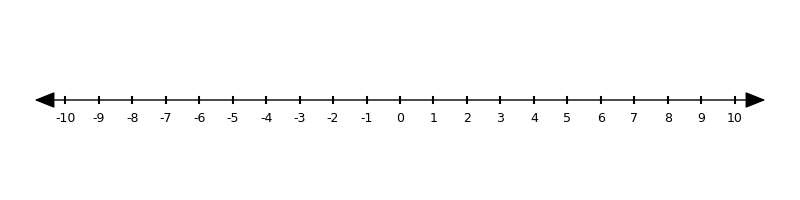
\includegraphics[keepaspectratio]{images/Unit_1/Lesson_1/blank_numberline.png}}

Here, every tick mark is an
\href{./glossary.html\#glossary-integer}{integer} --- a whole number.

\begin{itemize}
\tightlist
\item
  Numbers to the \textbf{right} of zero are \textbf{positive}
\item
  Numbers to the \textbf{left} of zero are \textbf{negative}
\end{itemize}

We can use this number line to \emph{see} what happens when we add,
subtract, or compare numbers.

\begin{tcolorbox}[enhanced jigsaw, opacityback=0, colframe=quarto-callout-note-color-frame, rightrule=.15mm, breakable, arc=.35mm, colback=white, leftrule=.75mm, toprule=.15mm, bottomrule=.15mm, left=2mm]

\vspace{-3mm}\textbf{🧠 How many numbers are between \(3\) and \(5\)?}\vspace{3mm}

The answer is not \(2\)! There are infinitely many numbers between \(3\)
and \(5\). Here are some number lines that might help convince you.

\pandocbounded{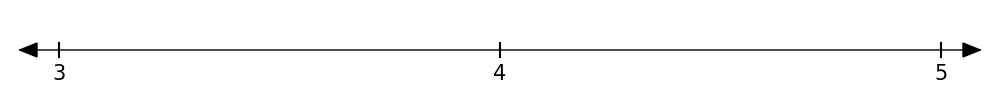
\includegraphics[keepaspectratio]{images/Unit_1/Lesson_1/three_to_five_by_1.png}}
\pandocbounded{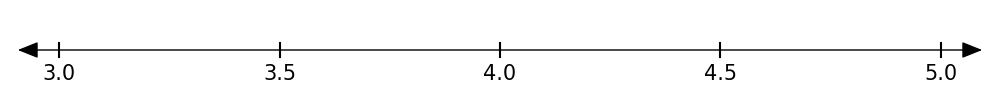
\includegraphics[keepaspectratio]{images/Unit_1/Lesson_1/between_3_and_5_by_05.png}}
\pandocbounded{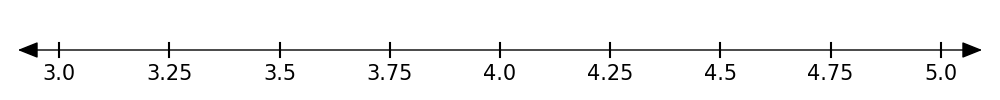
\includegraphics[keepaspectratio]{images/Unit_1/Lesson_1/between_3_and_5_by_025.png}}

\end{tcolorbox}

\subsection*{1.1.2 Understanding
Opposites}\label{understanding-opposites}
\addcontentsline{toc}{subsection}{1.1.2 Understanding Opposites}

Let's look at a pair of numbers, \(3\) and \(-3\).

These are called \href{./glossary.html\#glossary-opposite}{opposite}
numbers. They are the \textbf{same distance} from zero but on
\textbf{opposite sides} of it.

\pandocbounded{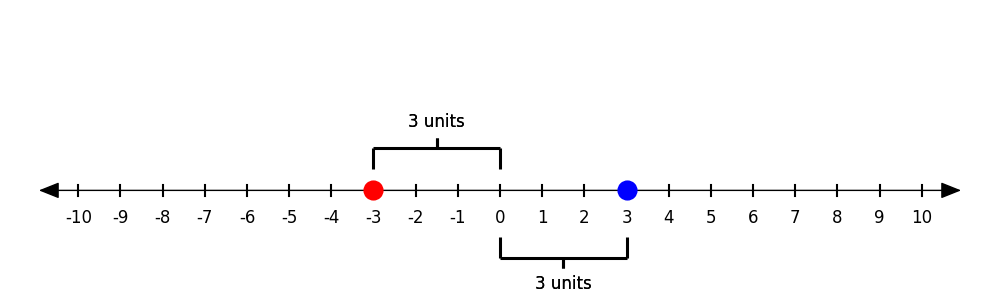
\includegraphics[keepaspectratio]{images/Unit_1/Lesson_1/opposites.png}}

\begin{tcolorbox}[enhanced jigsaw, opacityback=0, colframe=quarto-callout-note-color-frame, rightrule=.15mm, breakable, arc=.35mm, colback=white, leftrule=.75mm, toprule=.15mm, bottomrule=.15mm, left=2mm]

\vspace{-3mm}\textbf{🧠 What is the opposite of zero?}\vspace{3mm}

The opposite of zero is zero. Zero is the only number that is its own
opposite!

\end{tcolorbox}

\subsection*{1.1.3 What Is Absolute
Value?}\label{what-is-absolute-value}
\addcontentsline{toc}{subsection}{1.1.3 What Is Absolute Value?}

\href{./glossary.html\#glossary-absolute-value}{Absolute value}
(\(|x|\)) measures the \textbf{distance from zero}, no matter the
direction.

Take a look at the number \(-5\). The number line shows that it's
absolute value is \(5\) because it is \(5\) units away from zero.
\pandocbounded{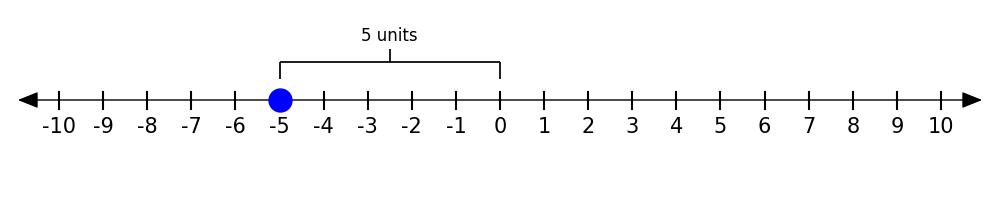
\includegraphics[keepaspectratio]{images/Unit_1/Lesson_1/absolute_value_negative_five.png}}

You can see that \(|5|\) is also \(5\) for the same reason!
\pandocbounded{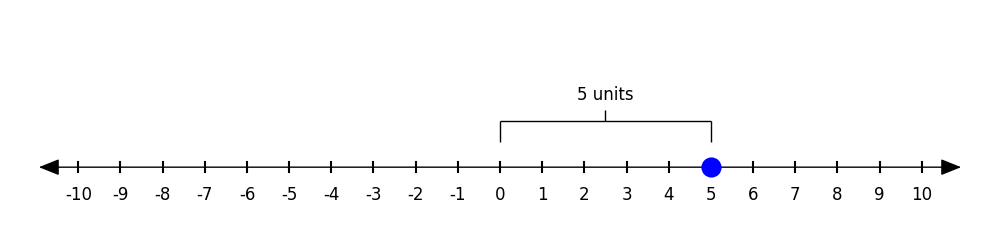
\includegraphics[keepaspectratio]{images/Unit_1/Lesson_1/absolute_value_five.png}}

\begin{tcolorbox}[enhanced jigsaw, opacityback=0, colframe=quarto-callout-note-color-frame, rightrule=.15mm, breakable, arc=.35mm, colback=white, leftrule=.75mm, toprule=.15mm, bottomrule=.15mm, left=2mm]

\vspace{-3mm}\textbf{🧠 Can the absolute value ever be negative?}\vspace{3mm}

Absolute value is \textbf{never} negative, because distance is never
negative.

\end{tcolorbox}

\begin{center}\rule{0.5\linewidth}{0.5pt}\end{center}

\subsection*{1.1.4 Comparing Integers}\label{comparing-integers}
\addcontentsline{toc}{subsection}{1.1.4 Comparing Integers}

We can also use the number line to compare values.

Let's compare \(2\) to \(-7\).
\pandocbounded{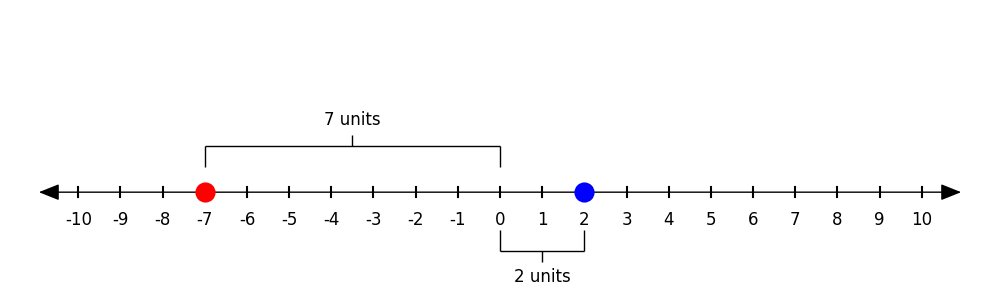
\includegraphics[keepaspectratio]{images/Unit_1/Lesson_1/compare_2_to_neg7.png}}

Ask yourself:

\begin{itemize}
\tightlist
\item
  Which number is farther \textbf{to the right}?
\item
  Which number is \textbf{closer to 0}?
\item
  Does absolute value change the comparison?
\end{itemize}

You can see from the number line that \(2 > -7\) because \(2\) is to the
right of \(-7\). But \(|-7|>|2|\), that is \(-7\) has a greater
\href{./glossary.html\#glossary-absolute-value}{absolute value} than
\(2\) because \(-7\) is further from zero.

\begin{tcolorbox}[enhanced jigsaw, opacityback=0, colframe=quarto-callout-note-color-frame, rightrule=.15mm, breakable, arc=.35mm, colback=white, leftrule=.75mm, toprule=.15mm, bottomrule=.15mm, left=2mm]

\vspace{-3mm}\textbf{🧠 Try comparing \(3\) to \(-8\) using a number line.}\vspace{3mm}

\(3 > -8\) because it is further to the right but \(|-8|>|3|\) because
\(-8\) is further from zero.

\pandocbounded{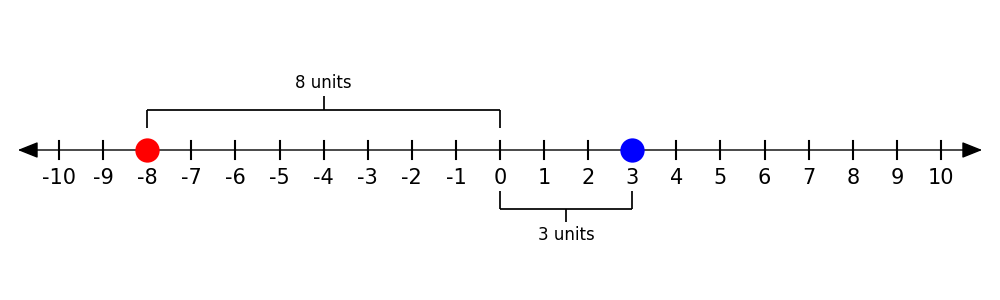
\includegraphics[keepaspectratio]{images/Unit_1/Lesson_1/compare_3_to_neg8.png}}

\end{tcolorbox}

\begin{center}\rule{0.5\linewidth}{0.5pt}\end{center}

\subsection*{1.1.5 Number Lines and
Arithmetic}\label{number-lines-and-arithmetic}
\addcontentsline{toc}{subsection}{1.1.5 Number Lines and Arithmetic}

We can also use the number line to model \textbf{adding and subtracting}
integers.

\begin{itemize}
\tightlist
\item
  To \textbf{add a positive number}, move \textbf{right}
\item
  To \textbf{add a negative number}, move \textbf{left}
\end{itemize}

Examples:

\begin{enumerate}
\def\labelenumi{\arabic{enumi}.}
\item
  Addition: \(-2 + 6 = 4\)
  \pandocbounded{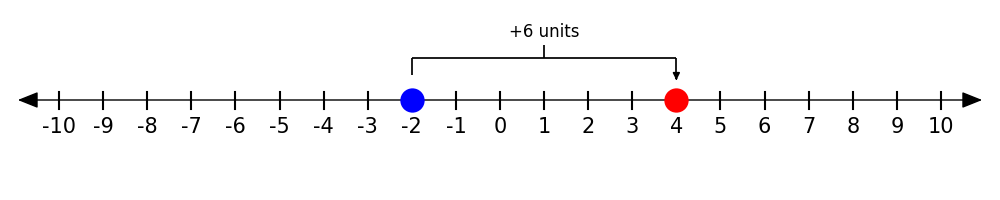
\includegraphics[keepaspectratio]{images/Unit_1/Lesson_1/add_6_to_neg2.png}}
\item
  Subtraction: \(4 - 7 = -3\)
  \pandocbounded{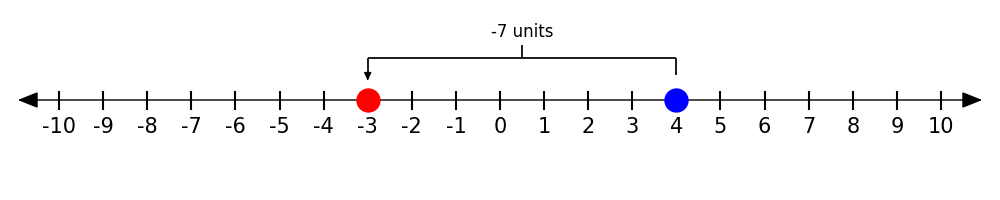
\includegraphics[keepaspectratio]{images/Unit_1/Lesson_1/subtract_7_from_4.png}}
\item
  Adding a negative: \(2 + (-5) = -3\)
  \pandocbounded{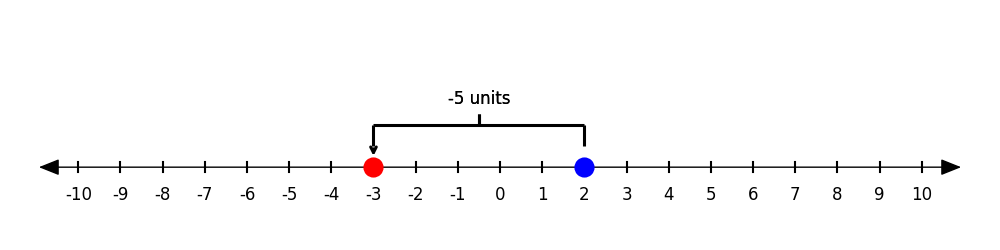
\includegraphics[keepaspectratio]{images/Unit_1/Lesson_1/add_neg5_to_2.png}}
\item
  Subtracting a negative: \(2 - (-3) = 5\)
  \pandocbounded{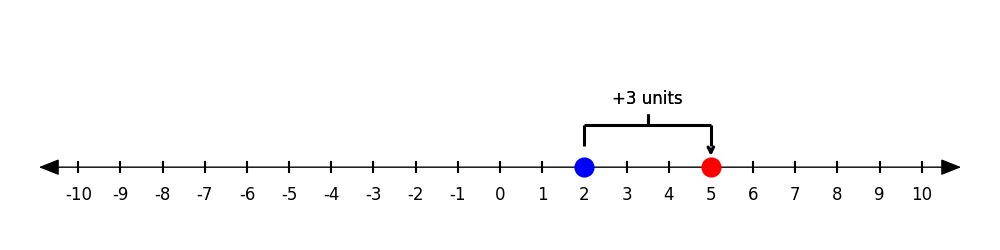
\includegraphics[keepaspectratio]{images/Unit_1/Lesson_1/subtract_neg3_from_2.png}}
\end{enumerate}

\begin{tcolorbox}[enhanced jigsaw, opacityback=0, colframe=quarto-callout-note-color-frame, rightrule=.15mm, breakable, arc=.35mm, colback=white, leftrule=.75mm, toprule=.15mm, bottomrule=.15mm, left=2mm]

\vspace{-3mm}\textbf{🧠 Can You think of a real-world example of each of these?}\vspace{3mm}

\begin{enumerate}
\def\labelenumi{\arabic{enumi}.}
\tightlist
\item
  You are \$\(2\) in debt and earn \$\(6\), now you have \$\(4\).
\item
  You have \$\(4\) and spend \$\(7\). You are now \$\(3\) in debt.
\item
  You have \$\(2\), the bank adds a \$\(5\) fee to your account. You now
  owe \$\(3\).
\item
  You have \$\(2\), the bank forgives a \$\(3\) overdraft fee. You now
  have \$\(5\).
\end{enumerate}

\end{tcolorbox}

\begin{center}\rule{0.5\linewidth}{0.5pt}\end{center}

\section*{✍️ Practice On Your Own}\label{practice-on-your-own}
\addcontentsline{toc}{section}{✍️ Practice On Your Own}

\markright{✍️ Practice On Your Own}

\subsection*{🧭 A. Locate and Label}\label{a.-locate-and-label}
\addcontentsline{toc}{subsection}{🧭 A. Locate and Label}

Plot the following integers on a number line: --10, --3, 0, 4, 9, --7

👉 \textbf{{[}INSERT: blank number line --12 to 12{]}}

\begin{center}\rule{0.5\linewidth}{0.5pt}\end{center}

\subsection*{🆚 B. Compare Using \textgreater, \textless, or
=}\label{b.-compare-using-or}
\addcontentsline{toc}{subsection}{🆚 B. Compare Using \textgreater,
\textless, or =}

\begin{enumerate}
\def\labelenumi{\arabic{enumi}.}
\tightlist
\item
  --4 \_\_\_ --9
\item
  --3 \_\_\_ 0
\item
  \textbar--5\textbar{} \_\_\_ 5
\item
  --\textbar--6\textbar{} \_\_\_ 6
\item
  --7 \_\_\_ --\textbar8\textbar{}
\item
  --2 -- 3 \_\_\_ --7
\item
  \textbar--3 -- 6\textbar{} \_\_\_ 9
\end{enumerate}

\begin{center}\rule{0.5\linewidth}{0.5pt}\end{center}

\subsection*{🔁 C. Opposites and Absolute
Value}\label{c.-opposites-and-absolute-value}
\addcontentsline{toc}{subsection}{🔁 C. Opposites and Absolute Value}

Fill in the blank:

\begin{enumerate}
\def\labelenumi{\arabic{enumi}.}
\tightlist
\item
  The opposite of --6 is \_\_\_
\item
  The opposite of 0 is \_\_\_
\item
  \textbar--12\textbar{} = \_\_\_
\item
  \textbar--3\textbar{} + \textbar--5\textbar{} = \_\_\_
\item
  --(--4) = \_\_\_
\item
  \textbar3 -- 9\textbar{} = \_\_\_
\end{enumerate}

\begin{center}\rule{0.5\linewidth}{0.5pt}\end{center}

\subsection*{⚖️ D. Reasoning Practice}\label{d.-reasoning-practice}
\addcontentsline{toc}{subsection}{⚖️ D. Reasoning Practice}

\textbf{True or False}? Justify with a sentence or sketch a number line.

\begin{enumerate}
\def\labelenumi{\arabic{enumi}.}
\tightlist
\item
  --3 \textgreater{} --9
\item
  \textbar--7\textbar{} = --\textbar7\textbar{}
\item
  The opposite of \textbar--5\textbar{} is --5
\item
  --(--8) = \textbar8\textbar{}
\end{enumerate}

\begin{center}\rule{0.5\linewidth}{0.5pt}\end{center}

\subsection*{🌡️ E. Contextual Word
Problems}\label{e.-contextual-word-problems}
\addcontentsline{toc}{subsection}{🌡️ E. Contextual Word Problems}

\begin{enumerate}
\def\labelenumi{\arabic{enumi}.}
\item
  The temperature was --12°F. It warmed up 20 degrees. What's the new
  temperature?
\item
  A diver is 45 feet below sea level. She goes down another 30 feet. How
  deep is she?
\item
  Your bank account is at --\$8. You deposit \$5. What's your new
  balance?
\end{enumerate}

\begin{center}\rule{0.5\linewidth}{0.5pt}\end{center}

\section*{✅ Answer Key (faded or
flipped)}\label{answer-key-faded-or-flipped}
\addcontentsline{toc}{section}{✅ Answer Key (faded or flipped)}

\markright{✅ Answer Key (faded or flipped)}

\begin{quote}
A: Labelled on number line B: \textgreater, \textless, =, \textless,
\textgreater, \textgreater, = C: 6, 0, 12, 8, 4, 6 D: T, F, F, T E: 8°F,
--75 ft, --\$3
\end{quote}

\begin{center}\rule{0.5\linewidth}{0.5pt}\end{center}

Would you like this exported as Quarto \texttt{.qmd} with stylized
headings, tooltips, and number line placeholders? I can also start
wiring in your plotting code or build a \texttt{.py} helper file with
reusable number line functions if you want this production-ready.

\chapter*{1.2 Factor Trees \& Prime
Factorization}\label{factor-trees-prime-factorization}
\addcontentsline{toc}{chapter}{1.2 Factor Trees \& Prime Factorization}

\markboth{1.2 Factor Trees \& Prime Factorization}{1.2 Factor Trees \&
Prime Factorization}

This lesson explores how to break numbers down into their prime
components using factor trees. Understanding prime factorization is key
for simplifying fractions and finding common factors.

\begin{tcolorbox}[enhanced jigsaw, colframe=quarto-callout-note-color-frame, opacitybacktitle=0.6, arc=.35mm, coltitle=black, leftrule=.75mm, toprule=.15mm, opacityback=0, bottomrule=.15mm, breakable, title={🎯 Objectives}, colback=white, bottomtitle=1mm, toptitle=1mm, titlerule=0mm, rightrule=.15mm, left=2mm, colbacktitle=quarto-callout-note-color!10!white]

\begin{itemize}
\tightlist
\item[$\square$]
  Identify prime numbers
\item[$\square$]
  Use factor trees to find the prime factorization of a number
\item[$\square$]
  Apply prime factorization in other math problems
\end{itemize}

\end{tcolorbox}

\begin{tcolorbox}[enhanced jigsaw, colframe=quarto-callout-note-color-frame, opacitybacktitle=0.6, arc=.35mm, coltitle=black, leftrule=.75mm, toprule=.15mm, opacityback=0, bottomrule=.15mm, breakable, title=\textcolor{quarto-callout-note-color}{\faInfo}\hspace{0.5em}{Vocabulary}, colback=white, bottomtitle=1mm, toptitle=1mm, titlerule=0mm, rightrule=.15mm, left=2mm, colbacktitle=quarto-callout-note-color!10!white]

prime, factor, factor tree, prime factorization

\end{tcolorbox}

\section*{🔥 Warm-Up}\label{warm-up-1}
\addcontentsline{toc}{section}{🔥 Warm-Up}

\markright{🔥 Warm-Up}

Coming soon.

\section*{🧠 Learn Together}\label{learn-together-1}
\addcontentsline{toc}{section}{🧠 Learn Together}

\markright{🧠 Learn Together}

Coming soon.

\section*{✏️ Practice On Your Own}\label{practice-on-your-own-1}
\addcontentsline{toc}{section}{✏️ Practice On Your Own}

\markright{✏️ Practice On Your Own}

Coming soon.

\chapter*{1.3 Greatest Common Factor
(GCF)}\label{greatest-common-factor-gcf}
\addcontentsline{toc}{chapter}{1.3 Greatest Common Factor (GCF)}

\markboth{1.3 Greatest Common Factor (GCF)}{1.3 Greatest Common Factor
(GCF)}

You'll learn how to find the GCF of two or more numbers using prime
factorization. GCF is important for simplifying fractions and solving
real-world problems involving multiples.

\begin{tcolorbox}[enhanced jigsaw, colframe=quarto-callout-note-color-frame, opacitybacktitle=0.6, arc=.35mm, coltitle=black, leftrule=.75mm, toprule=.15mm, opacityback=0, bottomrule=.15mm, breakable, title={🎯 Objectives}, colback=white, bottomtitle=1mm, toptitle=1mm, titlerule=0mm, rightrule=.15mm, left=2mm, colbacktitle=quarto-callout-note-color!10!white]

\begin{itemize}
\tightlist
\item[$\square$]
  Find the GCF using prime factorization
\item[$\square$]
  Apply GCF to simplify fractions
\item[$\square$]
  Solve problems involving shared quantities
\end{itemize}

\end{tcolorbox}

\begin{tcolorbox}[enhanced jigsaw, colframe=quarto-callout-note-color-frame, opacitybacktitle=0.6, arc=.35mm, coltitle=black, leftrule=.75mm, toprule=.15mm, opacityback=0, bottomrule=.15mm, breakable, title=\textcolor{quarto-callout-note-color}{\faInfo}\hspace{0.5em}{Vocabulary}, colback=white, bottomtitle=1mm, toptitle=1mm, titlerule=0mm, rightrule=.15mm, left=2mm, colbacktitle=quarto-callout-note-color!10!white]

GCF, common factor, prime factor, simplify

\end{tcolorbox}

\section*{🔥 Warm-Up}\label{warm-up-2}
\addcontentsline{toc}{section}{🔥 Warm-Up}

\markright{🔥 Warm-Up}

Coming soon.

\section*{🧠 Learn Together}\label{learn-together-2}
\addcontentsline{toc}{section}{🧠 Learn Together}

\markright{🧠 Learn Together}

Coming soon.

\section*{✏️ Practice On Your Own}\label{practice-on-your-own-2}
\addcontentsline{toc}{section}{✏️ Practice On Your Own}

\markright{✏️ Practice On Your Own}

Coming soon.

\chapter*{1.4 Multiplication \& Division
Fluency}\label{multiplication-division-fluency}
\addcontentsline{toc}{chapter}{1.4 Multiplication \& Division Fluency}

\markboth{1.4 Multiplication \& Division Fluency}{1.4 Multiplication \&
Division Fluency}

This lesson builds speed and accuracy with multiplication and division.
Being fluent in these operations will help with algebraic expressions
later.

\begin{tcolorbox}[enhanced jigsaw, colframe=quarto-callout-note-color-frame, opacitybacktitle=0.6, arc=.35mm, coltitle=black, leftrule=.75mm, toprule=.15mm, opacityback=0, bottomrule=.15mm, breakable, title={🎯 Objectives}, colback=white, bottomtitle=1mm, toptitle=1mm, titlerule=0mm, rightrule=.15mm, left=2mm, colbacktitle=quarto-callout-note-color!10!white]

\begin{itemize}
\tightlist
\item[$\square$]
  Practice multiplication facts
\item[$\square$]
  Practice division facts
\item[$\square$]
  Apply fluency to solve real problems
\end{itemize}

\end{tcolorbox}

\begin{tcolorbox}[enhanced jigsaw, colframe=quarto-callout-note-color-frame, opacitybacktitle=0.6, arc=.35mm, coltitle=black, leftrule=.75mm, toprule=.15mm, opacityback=0, bottomrule=.15mm, breakable, title=\textcolor{quarto-callout-note-color}{\faInfo}\hspace{0.5em}{Vocabulary}, colback=white, bottomtitle=1mm, toptitle=1mm, titlerule=0mm, rightrule=.15mm, left=2mm, colbacktitle=quarto-callout-note-color!10!white]

multiply, divide, fact family, quotient

\end{tcolorbox}

\section*{🔥 Warm-Up}\label{warm-up-3}
\addcontentsline{toc}{section}{🔥 Warm-Up}

\markright{🔥 Warm-Up}

Coming soon.

\section*{🧠 Learn Together}\label{learn-together-3}
\addcontentsline{toc}{section}{🧠 Learn Together}

\markright{🧠 Learn Together}

Coming soon.

\section*{✏️ Practice On Your Own}\label{practice-on-your-own-3}
\addcontentsline{toc}{section}{✏️ Practice On Your Own}

\markright{✏️ Practice On Your Own}

Coming soon.

\chapter*{1.5 Fractions: Meaning \&
Models}\label{fractions-meaning-models}
\addcontentsline{toc}{chapter}{1.5 Fractions: Meaning \& Models}

\markboth{1.5 Fractions: Meaning \& Models}{1.5 Fractions: Meaning \&
Models}

Learn what fractions represent and how to model them visually. This
lesson builds the foundational understanding needed for fraction
operations.

\begin{tcolorbox}[enhanced jigsaw, colframe=quarto-callout-note-color-frame, opacitybacktitle=0.6, arc=.35mm, coltitle=black, leftrule=.75mm, toprule=.15mm, opacityback=0, bottomrule=.15mm, breakable, title={🎯 Objectives}, colback=white, bottomtitle=1mm, toptitle=1mm, titlerule=0mm, rightrule=.15mm, left=2mm, colbacktitle=quarto-callout-note-color!10!white]

\begin{itemize}
\tightlist
\item[$\square$]
  Understand fractions as parts of a whole
\item[$\square$]
  Model fractions with shapes and number lines
\item[$\square$]
  Recognize proper and improper fractions
\end{itemize}

\end{tcolorbox}

\begin{tcolorbox}[enhanced jigsaw, colframe=quarto-callout-note-color-frame, opacitybacktitle=0.6, arc=.35mm, coltitle=black, leftrule=.75mm, toprule=.15mm, opacityback=0, bottomrule=.15mm, breakable, title=\textcolor{quarto-callout-note-color}{\faInfo}\hspace{0.5em}{Vocabulary}, colback=white, bottomtitle=1mm, toptitle=1mm, titlerule=0mm, rightrule=.15mm, left=2mm, colbacktitle=quarto-callout-note-color!10!white]

fraction, numerator, denominator, proper fraction, improper fraction

\end{tcolorbox}

\section*{🔥 Warm-Up}\label{warm-up-4}
\addcontentsline{toc}{section}{🔥 Warm-Up}

\markright{🔥 Warm-Up}

Coming soon.

\section*{🧠 Learn Together}\label{learn-together-4}
\addcontentsline{toc}{section}{🧠 Learn Together}

\markright{🧠 Learn Together}

Coming soon.

\section*{✏️ Practice On Your Own}\label{practice-on-your-own-4}
\addcontentsline{toc}{section}{✏️ Practice On Your Own}

\markright{✏️ Practice On Your Own}

Coming soon.

\chapter*{1.6 Simplifying Fractions Using
GCF}\label{simplifying-fractions-using-gcf}
\addcontentsline{toc}{chapter}{1.6 Simplifying Fractions Using GCF}

\markboth{1.6 Simplifying Fractions Using GCF}{1.6 Simplifying Fractions
Using GCF}

This lesson teaches how to simplify fractions by dividing the numerator
and denominator by their GCF.

\begin{tcolorbox}[enhanced jigsaw, colframe=quarto-callout-note-color-frame, opacitybacktitle=0.6, arc=.35mm, coltitle=black, leftrule=.75mm, toprule=.15mm, opacityback=0, bottomrule=.15mm, breakable, title={🎯 Objectives}, colback=white, bottomtitle=1mm, toptitle=1mm, titlerule=0mm, rightrule=.15mm, left=2mm, colbacktitle=quarto-callout-note-color!10!white]

\begin{itemize}
\tightlist
\item[$\square$]
  Simplify fractions using GCF
\item[$\square$]
  Recognize equivalent fractions
\item[$\square$]
  Use visual models to support simplification
\end{itemize}

\end{tcolorbox}

\begin{tcolorbox}[enhanced jigsaw, colframe=quarto-callout-note-color-frame, opacitybacktitle=0.6, arc=.35mm, coltitle=black, leftrule=.75mm, toprule=.15mm, opacityback=0, bottomrule=.15mm, breakable, title=\textcolor{quarto-callout-note-color}{\faInfo}\hspace{0.5em}{Vocabulary}, colback=white, bottomtitle=1mm, toptitle=1mm, titlerule=0mm, rightrule=.15mm, left=2mm, colbacktitle=quarto-callout-note-color!10!white]

simplify, equivalent, GCF, fraction

\end{tcolorbox}

\section*{🔥 Warm-Up}\label{warm-up-5}
\addcontentsline{toc}{section}{🔥 Warm-Up}

\markright{🔥 Warm-Up}

Coming soon.

\section*{🧠 Learn Together}\label{learn-together-5}
\addcontentsline{toc}{section}{🧠 Learn Together}

\markright{🧠 Learn Together}

Coming soon.

\section*{✏️ Practice On Your Own}\label{practice-on-your-own-5}
\addcontentsline{toc}{section}{✏️ Practice On Your Own}

\markright{✏️ Practice On Your Own}

Coming soon.

\chapter*{1.7 Mixed Numbers \& Improper
Fractions}\label{mixed-numbers-improper-fractions}
\addcontentsline{toc}{chapter}{1.7 Mixed Numbers \& Improper Fractions}

\markboth{1.7 Mixed Numbers \& Improper Fractions}{1.7 Mixed Numbers \&
Improper Fractions}

You'll learn how to convert between mixed numbers and improper
fractions, and why both forms are useful.

\begin{tcolorbox}[enhanced jigsaw, colframe=quarto-callout-note-color-frame, opacitybacktitle=0.6, arc=.35mm, coltitle=black, leftrule=.75mm, toprule=.15mm, opacityback=0, bottomrule=.15mm, breakable, title={🎯 Objectives}, colback=white, bottomtitle=1mm, toptitle=1mm, titlerule=0mm, rightrule=.15mm, left=2mm, colbacktitle=quarto-callout-note-color!10!white]

\begin{itemize}
\tightlist
\item[$\square$]
  Convert between mixed numbers and improper fractions
\item[$\square$]
  Visualize mixed numbers on number lines
\item[$\square$]
  Use both forms in real-world situations
\end{itemize}

\end{tcolorbox}

\begin{tcolorbox}[enhanced jigsaw, colframe=quarto-callout-note-color-frame, opacitybacktitle=0.6, arc=.35mm, coltitle=black, leftrule=.75mm, toprule=.15mm, opacityback=0, bottomrule=.15mm, breakable, title=\textcolor{quarto-callout-note-color}{\faInfo}\hspace{0.5em}{Vocabulary}, colback=white, bottomtitle=1mm, toptitle=1mm, titlerule=0mm, rightrule=.15mm, left=2mm, colbacktitle=quarto-callout-note-color!10!white]

mixed number, improper fraction, convert

\end{tcolorbox}

\section*{🔥 Warm-Up}\label{warm-up-6}
\addcontentsline{toc}{section}{🔥 Warm-Up}

\markright{🔥 Warm-Up}

Coming soon.

\section*{🧠 Learn Together}\label{learn-together-6}
\addcontentsline{toc}{section}{🧠 Learn Together}

\markright{🧠 Learn Together}

Coming soon.

\section*{✏️ Practice On Your Own}\label{practice-on-your-own-6}
\addcontentsline{toc}{section}{✏️ Practice On Your Own}

\markright{✏️ Practice On Your Own}

Coming soon.

\chapter*{1.8 Order of Operations}\label{order-of-operations}
\addcontentsline{toc}{chapter}{1.8 Order of Operations}

\markboth{1.8 Order of Operations}{1.8 Order of Operations}

In this lesson, we'll explore how to simplify expressions using the
correct order of operations (PEMDAS).

\begin{tcolorbox}[enhanced jigsaw, colframe=quarto-callout-note-color-frame, opacitybacktitle=0.6, arc=.35mm, coltitle=black, leftrule=.75mm, toprule=.15mm, opacityback=0, bottomrule=.15mm, breakable, title={🎯 Objectives}, colback=white, bottomtitle=1mm, toptitle=1mm, titlerule=0mm, rightrule=.15mm, left=2mm, colbacktitle=quarto-callout-note-color!10!white]

\begin{itemize}
\tightlist
\item[$\square$]
  Apply the order of operations to simplify expressions
\item[$\square$]
  Use grouping symbols correctly
\item[$\square$]
  Solve multi-step expressions
\end{itemize}

\end{tcolorbox}

\begin{tcolorbox}[enhanced jigsaw, colframe=quarto-callout-note-color-frame, opacitybacktitle=0.6, arc=.35mm, coltitle=black, leftrule=.75mm, toprule=.15mm, opacityback=0, bottomrule=.15mm, breakable, title=\textcolor{quarto-callout-note-color}{\faInfo}\hspace{0.5em}{Vocabulary}, colback=white, bottomtitle=1mm, toptitle=1mm, titlerule=0mm, rightrule=.15mm, left=2mm, colbacktitle=quarto-callout-note-color!10!white]

order of operations, PEMDAS, grouping symbols

\end{tcolorbox}

\section*{🔥 Warm-Up}\label{warm-up-7}
\addcontentsline{toc}{section}{🔥 Warm-Up}

\markright{🔥 Warm-Up}

Coming soon.

\section*{🧠 Learn Together}\label{learn-together-7}
\addcontentsline{toc}{section}{🧠 Learn Together}

\markright{🧠 Learn Together}

Coming soon.

\section*{✏️ Practice On Your Own}\label{practice-on-your-own-7}
\addcontentsline{toc}{section}{✏️ Practice On Your Own}

\markright{✏️ Practice On Your Own}

Coming soon.

\part{Unit 2: Algebraic Expressions}

\chapter*{Introduction}\label{introduction-1}
\addcontentsline{toc}{chapter}{Introduction}

\markboth{Introduction}{Introduction}

Lorem ipsum dolor sit amet, consectetur adipiscing elit. Duis sagittis
posuere ligula sit amet lacinia. Duis dignissim pellentesque magna,
rhoncus congue sapien finibus mollis. Ut eu sem laoreet, vehicula ipsum
in, convallis erat. Vestibulum magna sem, blandit pulvinar augue sit
amet, auctor malesuada sapien. Nullam faucibus leo eget eros hendrerit,
non laoreet ipsum lacinia. Curabitur cursus diam elit, non tempus ante
volutpat a. Quisque hendrerit blandit purus non fringilla. Integer sit
amet elit viverra ante dapibus semper. Vestibulum viverra rutrum enim,
at luctus enim posuere eu. Orci varius natoque penatibus et magnis dis
parturient montes, nascetur ridiculus mus.

Nunc ac dignissim magna. Vestibulum vitae egestas elit. Proin feugiat
leo quis ante condimentum, eu ornare mauris feugiat. Pellentesque
habitant morbi tristique senectus et netus et malesuada fames ac turpis
egestas. Mauris cursus laoreet ex, dignissim bibendum est posuere
iaculis. Suspendisse et maximus elit. In fringilla gravida ornare.
Aenean id lectus pulvinar, sagittis felis nec, rutrum risus. Nam vel
neque eu arcu blandit fringilla et in quam. Aliquam luctus est sit amet
vestibulum eleifend. Phasellus elementum sagittis molestie. Proin tempor
lorem arcu, at condimentum purus volutpat eu. Fusce et pellentesque
ligula. Pellentesque id tellus at erat luctus fringilla. Suspendisse
potenti.

Etiam maximus accumsan gravida. Maecenas at nunc dignissim, euismod enim
ac, bibendum ipsum. Maecenas vehicula velit in nisl aliquet ultricies.
Nam eget massa interdum, maximus arcu vel, pretium erat. Maecenas sit
amet tempor purus, vitae aliquet nunc. Vivamus cursus urna velit,
eleifend dictum magna laoreet ut. Duis eu erat mollis, blandit magna id,
tincidunt ipsum. Integer massa nibh, commodo eu ex vel, venenatis
efficitur ligula. Integer convallis lacus elit, maximus eleifend lacus
ornare ac. Vestibulum scelerisque viverra urna id lacinia. Vestibulum
ante ipsum primis in faucibus orci luctus et ultrices posuere cubilia
curae; Aenean eget enim at diam bibendum tincidunt eu non purus. Nullam
id magna ultrices, sodales metus viverra, tempus turpis.

\chapter*{2.1 Evaluating Expressions}\label{evaluating-expressions}
\addcontentsline{toc}{chapter}{2.1 Evaluating Expressions}

\markboth{2.1 Evaluating Expressions}{2.1 Evaluating Expressions}

You'll learn how to evaluate algebraic expressions by substituting
values for variables.

\begin{tcolorbox}[enhanced jigsaw, colframe=quarto-callout-note-color-frame, opacitybacktitle=0.6, arc=.35mm, coltitle=black, leftrule=.75mm, toprule=.15mm, opacityback=0, bottomrule=.15mm, breakable, title={🎯 Objectives}, colback=white, bottomtitle=1mm, toptitle=1mm, titlerule=0mm, rightrule=.15mm, left=2mm, colbacktitle=quarto-callout-note-color!10!white]

\begin{itemize}
\tightlist
\item[$\square$]
  Evaluate expressions with one or more variables
\item[$\square$]
  Use correct substitution and order
\item[$\square$]
  Check your work for accuracy
\end{itemize}

\end{tcolorbox}

\begin{tcolorbox}[enhanced jigsaw, colframe=quarto-callout-note-color-frame, opacitybacktitle=0.6, arc=.35mm, coltitle=black, leftrule=.75mm, toprule=.15mm, opacityback=0, bottomrule=.15mm, breakable, title=\textcolor{quarto-callout-note-color}{\faInfo}\hspace{0.5em}{Vocabulary}, colback=white, bottomtitle=1mm, toptitle=1mm, titlerule=0mm, rightrule=.15mm, left=2mm, colbacktitle=quarto-callout-note-color!10!white]

expression, evaluate, substitute, variable

\end{tcolorbox}

\section*{🔥 Warm-Up}\label{warm-up-8}
\addcontentsline{toc}{section}{🔥 Warm-Up}

\markright{🔥 Warm-Up}

Coming soon.

\section*{🧠 Learn Together}\label{learn-together-8}
\addcontentsline{toc}{section}{🧠 Learn Together}

\markright{🧠 Learn Together}

Coming soon.

\section*{✏️ Practice On Your Own}\label{practice-on-your-own-8}
\addcontentsline{toc}{section}{✏️ Practice On Your Own}

\markright{✏️ Practice On Your Own}

Coming soon.

\chapter*{2.2 Inputs, Outputs \& Function Machines
(Intro)}\label{inputs-outputs-function-machines-intro}
\addcontentsline{toc}{chapter}{2.2 Inputs, Outputs \& Function Machines
(Intro)}

\markboth{2.2 Inputs, Outputs \& Function Machines (Intro)}{2.2 Inputs,
Outputs \& Function Machines (Intro)}

This introductory lesson explains how functions work using simple
input-output models. This is the foundation for understanding functions
throughout the course.

\begin{tcolorbox}[enhanced jigsaw, colframe=quarto-callout-note-color-frame, opacitybacktitle=0.6, arc=.35mm, coltitle=black, leftrule=.75mm, toprule=.15mm, opacityback=0, bottomrule=.15mm, breakable, title={🎯 Objectives}, colback=white, bottomtitle=1mm, toptitle=1mm, titlerule=0mm, rightrule=.15mm, left=2mm, colbacktitle=quarto-callout-note-color!10!white]

\begin{itemize}
\tightlist
\item[$\square$]
  Understand the concept of a function
\item[$\square$]
  Match inputs with outputs
\item[$\square$]
  Identify function rules from patterns
\end{itemize}

\end{tcolorbox}

\begin{tcolorbox}[enhanced jigsaw, colframe=quarto-callout-note-color-frame, opacitybacktitle=0.6, arc=.35mm, coltitle=black, leftrule=.75mm, toprule=.15mm, opacityback=0, bottomrule=.15mm, breakable, title=\textcolor{quarto-callout-note-color}{\faInfo}\hspace{0.5em}{Vocabulary}, colback=white, bottomtitle=1mm, toptitle=1mm, titlerule=0mm, rightrule=.15mm, left=2mm, colbacktitle=quarto-callout-note-color!10!white]

input, output, function, function rule

\end{tcolorbox}

\section*{🔥 Warm-Up}\label{warm-up-9}
\addcontentsline{toc}{section}{🔥 Warm-Up}

\markright{🔥 Warm-Up}

Coming soon.

\section*{🧠 Learn Together}\label{learn-together-9}
\addcontentsline{toc}{section}{🧠 Learn Together}

\markright{🧠 Learn Together}

Coming soon.

\section*{✏️ Practice On Your Own}\label{practice-on-your-own-9}
\addcontentsline{toc}{section}{✏️ Practice On Your Own}

\markright{✏️ Practice On Your Own}

Coming soon.

\part{Unit 3: Solving Equations}

\chapter*{Introduction}\label{introduction-2}
\addcontentsline{toc}{chapter}{Introduction}

\markboth{Introduction}{Introduction}

This unit is where Algebra really begins to feel like solving puzzles.
You'll learn how to isolate variables, understand balance, and make
sense of problems that come up in everyday life.

\begin{center}\rule{0.5\linewidth}{0.5pt}\end{center}

\section*{What You'll Learn}\label{what-youll-learn-1}
\addcontentsline{toc}{section}{What You'll Learn}

\markright{What You'll Learn}

By the end of this unit, you'll be able to:

\begin{itemize}
\tightlist
\item
  Solve one- and two-step equations using inverse operations
\item
  Distribute and combine like terms in multi-step equations
\item
  Move variables to one side of the equation
\item
  Identify when equations have no or infinite solutions
\item
  Write and solve equations from word problems and contexts
\end{itemize}

\begin{center}\rule{0.5\linewidth}{0.5pt}\end{center}

\section*{📦 Topics in This Unit}\label{topics-in-this-unit-1}
\addcontentsline{toc}{section}{📦 Topics in This Unit}

\markright{📦 Topics in This Unit}

\subsection*{3. Solving One- and Two-Step
Equations}\label{solving-one--and-two-step-equations}
\addcontentsline{toc}{subsection}{3. Solving One- and Two-Step
Equations}

Use inverse operations to find solutions.

\subsection*{3. Multi-Step Equations with
Distribution}\label{multi-step-equations-with-distribution}
\addcontentsline{toc}{subsection}{3. Multi-Step Equations with
Distribution}

Distribute, simplify, and solve more complex equations.

\subsection*{3. Equations with Variables on Both
Sides}\label{equations-with-variables-on-both-sides}
\addcontentsline{toc}{subsection}{3. Equations with Variables on Both
Sides}

Move all variable terms to one side, then solve.

\subsection*{3. No Solution vs.~Infinite
Solutions}\label{no-solution-vs.-infinite-solutions}
\addcontentsline{toc}{subsection}{3. No Solution vs.~Infinite Solutions}

Learn to recognize when an equation has no solution or all numbers work.

\subsection*{3. Writing Equations from
Contexts}\label{writing-equations-from-contexts}
\addcontentsline{toc}{subsection}{3. Writing Equations from Contexts}

Translate real-world problems into equations.

\subsection*{3. Solving with Tables, Graphs \&
Rules}\label{solving-with-tables-graphs-rules}
\addcontentsline{toc}{subsection}{3. Solving with Tables, Graphs \&
Rules}

Connect functions to equations and problem-solving.

\begin{center}\rule{0.5\linewidth}{0.5pt}\end{center}

\section*{🧭 How to Use This Unit}\label{how-to-use-this-unit}
\addcontentsline{toc}{section}{🧭 How to Use This Unit}

\markright{🧭 How to Use This Unit}

You'll find plenty of examples, visuals, and practice to help you
develop confidence in solving equations from both numbers and words!

\chapter*{3.1 Solving One-Step \& Two-Step
Equations}\label{solving-one-step-two-step-equations}
\addcontentsline{toc}{chapter}{3.1 Solving One-Step \& Two-Step
Equations}

\markboth{3.1 Solving One-Step \& Two-Step Equations}{3.1 Solving
One-Step \& Two-Step Equations}

In this lesson, students will learn how to solve one-step and two-step
equations using inverse operations. This foundational skill sets the
stage for solving more complex equations in future lessons.

\begin{tcolorbox}[enhanced jigsaw, colframe=quarto-callout-note-color-frame, opacitybacktitle=0.6, arc=.35mm, coltitle=black, leftrule=.75mm, toprule=.15mm, opacityback=0, bottomrule=.15mm, breakable, title={🎯 Objectives}, colback=white, bottomtitle=1mm, toptitle=1mm, titlerule=0mm, rightrule=.15mm, left=2mm, colbacktitle=quarto-callout-note-color!10!white]

\begin{itemize}
\tightlist
\item[$\square$]
  Use inverse operations to isolate the variable
\item[$\square$]
  Solve one-step and two-step equations involving addition, subtraction,
  multiplication, or division
\item[$\square$]
  Check solutions by substitution
\end{itemize}

\end{tcolorbox}

\begin{tcolorbox}[enhanced jigsaw, colframe=quarto-callout-note-color-frame, opacitybacktitle=0.6, arc=.35mm, coltitle=black, leftrule=.75mm, toprule=.15mm, opacityback=0, bottomrule=.15mm, breakable, title=\textcolor{quarto-callout-note-color}{\faInfo}\hspace{0.5em}{Vocabulary}, colback=white, bottomtitle=1mm, toptitle=1mm, titlerule=0mm, rightrule=.15mm, left=2mm, colbacktitle=quarto-callout-note-color!10!white]

equation, inverse operations, solution, variable

\end{tcolorbox}

\section*{🔥 Warm-Up}\label{warm-up-10}
\addcontentsline{toc}{section}{🔥 Warm-Up}

\markright{🔥 Warm-Up}

Coming soon.

\section*{🧠 Learn Together}\label{learn-together-10}
\addcontentsline{toc}{section}{🧠 Learn Together}

\markright{🧠 Learn Together}

Coming soon.

\section*{✏️ Practice On Your Own}\label{practice-on-your-own-10}
\addcontentsline{toc}{section}{✏️ Practice On Your Own}

\markright{✏️ Practice On Your Own}

Coming soon.

\chapter*{3.2 Multi-Step Equations with
Distribution}\label{multi-step-equations-with-distribution-1}
\addcontentsline{toc}{chapter}{3.2 Multi-Step Equations with
Distribution}

\markboth{3.2 Multi-Step Equations with Distribution}{3.2 Multi-Step
Equations with Distribution}

This lesson extends equation solving to multi-step problems, including
those that require the distributive property and combining like terms.

\begin{tcolorbox}[enhanced jigsaw, colframe=quarto-callout-note-color-frame, opacitybacktitle=0.6, arc=.35mm, coltitle=black, leftrule=.75mm, toprule=.15mm, opacityback=0, bottomrule=.15mm, breakable, title={🎯 Objectives}, colback=white, bottomtitle=1mm, toptitle=1mm, titlerule=0mm, rightrule=.15mm, left=2mm, colbacktitle=quarto-callout-note-color!10!white]

\begin{itemize}
\tightlist
\item[$\square$]
  Apply the distributive property to simplify equations
\item[$\square$]
  Combine like terms before solving
\item[$\square$]
  Solve multi-step equations with multiple operations
\end{itemize}

\end{tcolorbox}

\begin{tcolorbox}[enhanced jigsaw, colframe=quarto-callout-note-color-frame, opacitybacktitle=0.6, arc=.35mm, coltitle=black, leftrule=.75mm, toprule=.15mm, opacityback=0, bottomrule=.15mm, breakable, title=\textcolor{quarto-callout-note-color}{\faInfo}\hspace{0.5em}{Vocabulary}, colback=white, bottomtitle=1mm, toptitle=1mm, titlerule=0mm, rightrule=.15mm, left=2mm, colbacktitle=quarto-callout-note-color!10!white]

distributive property, like terms, combine, simplify

\end{tcolorbox}

\section*{🔥 Warm-Up}\label{warm-up-11}
\addcontentsline{toc}{section}{🔥 Warm-Up}

\markright{🔥 Warm-Up}

Coming soon.

\section*{🧠 Learn Together}\label{learn-together-11}
\addcontentsline{toc}{section}{🧠 Learn Together}

\markright{🧠 Learn Together}

Coming soon.

\section*{✏️ Practice On Your Own}\label{practice-on-your-own-11}
\addcontentsline{toc}{section}{✏️ Practice On Your Own}

\markright{✏️ Practice On Your Own}

Coming soon.

\chapter*{3.3 Equations with Variables on Both
Sides}\label{equations-with-variables-on-both-sides-1}
\addcontentsline{toc}{chapter}{3.3 Equations with Variables on Both
Sides}

\markboth{3.3 Equations with Variables on Both Sides}{3.3 Equations with
Variables on Both Sides}

Students will learn how to solve equations where variables appear on
both sides of the equals sign, reinforcing the concept of balancing and
simplifying equations.

\begin{tcolorbox}[enhanced jigsaw, colframe=quarto-callout-note-color-frame, opacitybacktitle=0.6, arc=.35mm, coltitle=black, leftrule=.75mm, toprule=.15mm, opacityback=0, bottomrule=.15mm, breakable, title={🎯 Objectives}, colback=white, bottomtitle=1mm, toptitle=1mm, titlerule=0mm, rightrule=.15mm, left=2mm, colbacktitle=quarto-callout-note-color!10!white]

\begin{itemize}
\tightlist
\item[$\square$]
  Move variable terms to one side of the equation
\item[$\square$]
  Simplify both sides before solving
\item[$\square$]
  Identify equations with no or infinite solutions
\end{itemize}

\end{tcolorbox}

\begin{tcolorbox}[enhanced jigsaw, colframe=quarto-callout-note-color-frame, opacitybacktitle=0.6, arc=.35mm, coltitle=black, leftrule=.75mm, toprule=.15mm, opacityback=0, bottomrule=.15mm, breakable, title=\textcolor{quarto-callout-note-color}{\faInfo}\hspace{0.5em}{Vocabulary}, colback=white, bottomtitle=1mm, toptitle=1mm, titlerule=0mm, rightrule=.15mm, left=2mm, colbacktitle=quarto-callout-note-color!10!white]

combine like terms, variable, no solution, infinite solutions

\end{tcolorbox}

\section*{🔥 Warm-Up}\label{warm-up-12}
\addcontentsline{toc}{section}{🔥 Warm-Up}

\markright{🔥 Warm-Up}

Coming soon.

\section*{🧠 Learn Together}\label{learn-together-12}
\addcontentsline{toc}{section}{🧠 Learn Together}

\markright{🧠 Learn Together}

Coming soon.

\section*{✏️ Practice On Your Own}\label{practice-on-your-own-12}
\addcontentsline{toc}{section}{✏️ Practice On Your Own}

\markright{✏️ Practice On Your Own}

Coming soon.

\chapter*{3.4 No Solution vs.~Infinite
Solutions}\label{no-solution-vs.-infinite-solutions-1}
\addcontentsline{toc}{chapter}{3.4 No Solution vs.~Infinite Solutions}

\markboth{3.4 No Solution vs.~Infinite Solutions}{3.4 No Solution
vs.~Infinite Solutions}

This lesson focuses on identifying when equations have no solution or
infinitely many solutions and how to justify those conclusions.

\begin{tcolorbox}[enhanced jigsaw, colframe=quarto-callout-note-color-frame, opacitybacktitle=0.6, arc=.35mm, coltitle=black, leftrule=.75mm, toprule=.15mm, opacityback=0, bottomrule=.15mm, breakable, title={🎯 Objectives}, colback=white, bottomtitle=1mm, toptitle=1mm, titlerule=0mm, rightrule=.15mm, left=2mm, colbacktitle=quarto-callout-note-color!10!white]

\begin{itemize}
\tightlist
\item[$\square$]
  Recognize inconsistent equations with no solution
\item[$\square$]
  Identify dependent equations with infinite solutions
\item[$\square$]
  Justify solutions using substitution or reasoning
\end{itemize}

\end{tcolorbox}

\begin{tcolorbox}[enhanced jigsaw, colframe=quarto-callout-note-color-frame, opacitybacktitle=0.6, arc=.35mm, coltitle=black, leftrule=.75mm, toprule=.15mm, opacityback=0, bottomrule=.15mm, breakable, title=\textcolor{quarto-callout-note-color}{\faInfo}\hspace{0.5em}{Vocabulary}, colback=white, bottomtitle=1mm, toptitle=1mm, titlerule=0mm, rightrule=.15mm, left=2mm, colbacktitle=quarto-callout-note-color!10!white]

identity, contradiction, solution set, consistent, inconsistent

\end{tcolorbox}

\section*{🔥 Warm-Up}\label{warm-up-13}
\addcontentsline{toc}{section}{🔥 Warm-Up}

\markright{🔥 Warm-Up}

Coming soon.

\section*{🧠 Learn Together}\label{learn-together-13}
\addcontentsline{toc}{section}{🧠 Learn Together}

\markright{🧠 Learn Together}

Coming soon.

\section*{✏️ Practice On Your Own}\label{practice-on-your-own-13}
\addcontentsline{toc}{section}{✏️ Practice On Your Own}

\markright{✏️ Practice On Your Own}

Coming soon.

\chapter*{3.5 Writing Equations from Real-Life
Contexts}\label{writing-equations-from-real-life-contexts}
\addcontentsline{toc}{chapter}{3.5 Writing Equations from Real-Life
Contexts}

\markboth{3.5 Writing Equations from Real-Life Contexts}{3.5 Writing
Equations from Real-Life Contexts}

Students will translate real-world scenarios into algebraic equations,
helping them understand the connection between math and everyday problem
solving.

\begin{tcolorbox}[enhanced jigsaw, colframe=quarto-callout-note-color-frame, opacitybacktitle=0.6, arc=.35mm, coltitle=black, leftrule=.75mm, toprule=.15mm, opacityback=0, bottomrule=.15mm, breakable, title={🎯 Objectives}, colback=white, bottomtitle=1mm, toptitle=1mm, titlerule=0mm, rightrule=.15mm, left=2mm, colbacktitle=quarto-callout-note-color!10!white]

\begin{itemize}
\tightlist
\item[$\square$]
  Identify quantities and relationships in word problems
\item[$\square$]
  Write algebraic equations to represent situations
\item[$\square$]
  Solve and interpret solutions in context
\end{itemize}

\end{tcolorbox}

\begin{tcolorbox}[enhanced jigsaw, colframe=quarto-callout-note-color-frame, opacitybacktitle=0.6, arc=.35mm, coltitle=black, leftrule=.75mm, toprule=.15mm, opacityback=0, bottomrule=.15mm, breakable, title=\textcolor{quarto-callout-note-color}{\faInfo}\hspace{0.5em}{Vocabulary}, colback=white, bottomtitle=1mm, toptitle=1mm, titlerule=0mm, rightrule=.15mm, left=2mm, colbacktitle=quarto-callout-note-color!10!white]

context, representation, translate, real-world

\end{tcolorbox}

\section*{🔥 Warm-Up}\label{warm-up-14}
\addcontentsline{toc}{section}{🔥 Warm-Up}

\markright{🔥 Warm-Up}

Coming soon.

\section*{🧠 Learn Together}\label{learn-together-14}
\addcontentsline{toc}{section}{🧠 Learn Together}

\markright{🧠 Learn Together}

Coming soon.

\section*{✏️ Practice On Your Own}\label{practice-on-your-own-14}
\addcontentsline{toc}{section}{✏️ Practice On Your Own}

\markright{✏️ Practice On Your Own}

Coming soon.

\chapter*{3.6 Solving with Tables, Graphs \& Rules (Function
Tie-In)}\label{solving-with-tables-graphs-rules-function-tie-in}
\addcontentsline{toc}{chapter}{3.6 Solving with Tables, Graphs \& Rules
(Function Tie-In)}

\markboth{3.6 Solving with Tables, Graphs \& Rules (Function
Tie-In)}{3.6 Solving with Tables, Graphs \& Rules (Function Tie-In)}

This lesson introduces multiple representations of relationships ---
including tables, graphs, and rules --- to show how equations can be
connected to functions.

\begin{tcolorbox}[enhanced jigsaw, colframe=quarto-callout-note-color-frame, opacitybacktitle=0.6, arc=.35mm, coltitle=black, leftrule=.75mm, toprule=.15mm, opacityback=0, bottomrule=.15mm, breakable, title={🎯 Objectives}, colback=white, bottomtitle=1mm, toptitle=1mm, titlerule=0mm, rightrule=.15mm, left=2mm, colbacktitle=quarto-callout-note-color!10!white]

\begin{itemize}
\tightlist
\item[$\square$]
  Solve equations by analyzing input-output tables
\item[$\square$]
  Interpret relationships from graphs and equations
\item[$\square$]
  Connect equations to real-world patterns
\end{itemize}

\end{tcolorbox}

\begin{tcolorbox}[enhanced jigsaw, colframe=quarto-callout-note-color-frame, opacitybacktitle=0.6, arc=.35mm, coltitle=black, leftrule=.75mm, toprule=.15mm, opacityback=0, bottomrule=.15mm, breakable, title=\textcolor{quarto-callout-note-color}{\faInfo}\hspace{0.5em}{Vocabulary}, colback=white, bottomtitle=1mm, toptitle=1mm, titlerule=0mm, rightrule=.15mm, left=2mm, colbacktitle=quarto-callout-note-color!10!white]

input, output, table, function, rule, graph

\end{tcolorbox}

\section*{🔥 Warm-Up}\label{warm-up-15}
\addcontentsline{toc}{section}{🔥 Warm-Up}

\markright{🔥 Warm-Up}

Coming soon.

\section*{🧠 Learn Together}\label{learn-together-15}
\addcontentsline{toc}{section}{🧠 Learn Together}

\markright{🧠 Learn Together}

Coming soon.

\section*{✏️ Practice On Your Own}\label{practice-on-your-own-15}
\addcontentsline{toc}{section}{✏️ Practice On Your Own}

\markright{✏️ Practice On Your Own}

Coming soon.

\part{Unit 4: Graphs and Patterns}

\chapter*{Introduction}\label{introduction-3}
\addcontentsline{toc}{chapter}{Introduction}

\markboth{Introduction}{Introduction}

In this unit, we'll use visual and numerical patterns to understand how
algebraic relationships behave. This helps us prepare for graphing and
working with functions in more depth.

\begin{center}\rule{0.5\linewidth}{0.5pt}\end{center}

\section*{What You'll Learn}\label{what-youll-learn-2}
\addcontentsline{toc}{section}{What You'll Learn}

\markright{What You'll Learn}

\begin{itemize}
\tightlist
\item
  Recognize and extend arithmetic and geometric patterns
\item
  Build and interpret tables
\item
  Graph expressions and equations
\item
  Compare linear models using graphs
\end{itemize}

\begin{center}\rule{0.5\linewidth}{0.5pt}\end{center}

\section*{📦 Topics in This Unit}\label{topics-in-this-unit-2}
\addcontentsline{toc}{section}{📦 Topics in This Unit}

\markright{📦 Topics in This Unit}

\subsection*{4. Graphing Expressions with
Tables}\label{graphing-expressions-with-tables}
\addcontentsline{toc}{subsection}{4. Graphing Expressions with Tables}

Use input-output tables to generate points.

\subsection*{4. Interpreting Graphs in
Context}\label{interpreting-graphs-in-context}
\addcontentsline{toc}{subsection}{4. Interpreting Graphs in Context}

Make sense of graphs in stories and real-life settings.

\subsection*{4. Arithmetic vs.~Geometric
Patterns}\label{arithmetic-vs.-geometric-patterns}
\addcontentsline{toc}{subsection}{4. Arithmetic vs.~Geometric Patterns}

Identify whether change is constant or multiplicative.

\subsection*{4. Linear Modeling \& Rate of
Change}\label{linear-modeling-rate-of-change}
\addcontentsline{toc}{subsection}{4. Linear Modeling \& Rate of Change}

Build linear functions and interpret slope in context.

\subsection*{4. Estimating and Checking with
Graphs}\label{estimating-and-checking-with-graphs}
\addcontentsline{toc}{subsection}{4. Estimating and Checking with
Graphs}

Use visuals to verify solutions.

\begin{center}\rule{0.5\linewidth}{0.5pt}\end{center}

\section*{🧭 How to Use This Unit}\label{how-to-use-this-unit-1}
\addcontentsline{toc}{section}{🧭 How to Use This Unit}

\markright{🧭 How to Use This Unit}

Graphing builds a strong link between abstract algebra and concrete
understanding. Let's get visual!

\chapter*{4.1 Graphing Expressions with
Tables}\label{graphing-expressions-with-tables-1}
\addcontentsline{toc}{chapter}{4.1 Graphing Expressions with Tables}

\markboth{4.1 Graphing Expressions with Tables}{4.1 Graphing Expressions
with Tables}

In this lesson, students will learn how to create tables of values for
algebraic expressions and plot them on a coordinate plane. This builds
foundational understanding of how algebraic rules connect to visual
patterns.

\begin{tcolorbox}[enhanced jigsaw, colframe=quarto-callout-note-color-frame, opacitybacktitle=0.6, arc=.35mm, coltitle=black, leftrule=.75mm, toprule=.15mm, opacityback=0, bottomrule=.15mm, breakable, title={🎯 Objectives}, colback=white, bottomtitle=1mm, toptitle=1mm, titlerule=0mm, rightrule=.15mm, left=2mm, colbacktitle=quarto-callout-note-color!10!white]

\begin{itemize}
\tightlist
\item[$\square$]
  Generate tables of values from algebraic expressions
\item[$\square$]
  Graph ordered pairs on the coordinate plane
\item[$\square$]
  Recognize linear patterns in tables and graphs
\end{itemize}

\end{tcolorbox}

\begin{tcolorbox}[enhanced jigsaw, colframe=quarto-callout-note-color-frame, opacitybacktitle=0.6, arc=.35mm, coltitle=black, leftrule=.75mm, toprule=.15mm, opacityback=0, bottomrule=.15mm, breakable, title=\textcolor{quarto-callout-note-color}{\faInfo}\hspace{0.5em}{Vocabulary}, colback=white, bottomtitle=1mm, toptitle=1mm, titlerule=0mm, rightrule=.15mm, left=2mm, colbacktitle=quarto-callout-note-color!10!white]

expression, table, ordered pair, coordinate plane, input, output

\end{tcolorbox}

\section*{🔥 Warm-Up}\label{warm-up-16}
\addcontentsline{toc}{section}{🔥 Warm-Up}

\markright{🔥 Warm-Up}

Coming soon.

\section*{🧠 Learn Together}\label{learn-together-16}
\addcontentsline{toc}{section}{🧠 Learn Together}

\markright{🧠 Learn Together}

Coming soon.

\section*{✏️ Practice On Your Own}\label{practice-on-your-own-16}
\addcontentsline{toc}{section}{✏️ Practice On Your Own}

\markright{✏️ Practice On Your Own}

Coming soon.

\chapter*{4.2 Interpreting Graphs in
Context}\label{interpreting-graphs-in-context-1}
\addcontentsline{toc}{chapter}{4.2 Interpreting Graphs in Context}

\markboth{4.2 Interpreting Graphs in Context}{4.2 Interpreting Graphs in
Context}

Students will examine graphs that represent real-world scenarios and
learn how to describe the relationships shown. Emphasis is placed on
labeling axes, identifying trends, and understanding what changes in
slope mean.

\begin{tcolorbox}[enhanced jigsaw, colframe=quarto-callout-note-color-frame, opacitybacktitle=0.6, arc=.35mm, coltitle=black, leftrule=.75mm, toprule=.15mm, opacityback=0, bottomrule=.15mm, breakable, title={🎯 Objectives}, colback=white, bottomtitle=1mm, toptitle=1mm, titlerule=0mm, rightrule=.15mm, left=2mm, colbacktitle=quarto-callout-note-color!10!white]

\begin{itemize}
\tightlist
\item[$\square$]
  Identify variables and units from graph labels
\item[$\square$]
  Describe trends in linear graphs
\item[$\square$]
  Interpret slope and intercepts in context
\end{itemize}

\end{tcolorbox}

\begin{tcolorbox}[enhanced jigsaw, colframe=quarto-callout-note-color-frame, opacitybacktitle=0.6, arc=.35mm, coltitle=black, leftrule=.75mm, toprule=.15mm, opacityback=0, bottomrule=.15mm, breakable, title=\textcolor{quarto-callout-note-color}{\faInfo}\hspace{0.5em}{Vocabulary}, colback=white, bottomtitle=1mm, toptitle=1mm, titlerule=0mm, rightrule=.15mm, left=2mm, colbacktitle=quarto-callout-note-color!10!white]

x-axis, y-axis, slope, intercept, context, trend

\end{tcolorbox}

\section*{🔥 Warm-Up}\label{warm-up-17}
\addcontentsline{toc}{section}{🔥 Warm-Up}

\markright{🔥 Warm-Up}

Coming soon.

\section*{🧠 Learn Together}\label{learn-together-17}
\addcontentsline{toc}{section}{🧠 Learn Together}

\markright{🧠 Learn Together}

Coming soon.

\section*{✏️ Practice On Your Own}\label{practice-on-your-own-17}
\addcontentsline{toc}{section}{✏️ Practice On Your Own}

\markright{✏️ Practice On Your Own}

Coming soon.

\chapter*{4.3 Arithmetic vs.~Geometric
Patterns}\label{arithmetic-vs.-geometric-patterns-1}
\addcontentsline{toc}{chapter}{4.3 Arithmetic vs.~Geometric Patterns}

\markboth{4.3 Arithmetic vs.~Geometric Patterns}{4.3 Arithmetic
vs.~Geometric Patterns}

Students will compare arithmetic and geometric patterns and recognize
how they grow. This helps build pattern recognition and introduces
exponential growth.

\begin{tcolorbox}[enhanced jigsaw, colframe=quarto-callout-note-color-frame, opacitybacktitle=0.6, arc=.35mm, coltitle=black, leftrule=.75mm, toprule=.15mm, opacityback=0, bottomrule=.15mm, breakable, title={🎯 Objectives}, colback=white, bottomtitle=1mm, toptitle=1mm, titlerule=0mm, rightrule=.15mm, left=2mm, colbacktitle=quarto-callout-note-color!10!white]

\begin{itemize}
\tightlist
\item[$\square$]
  Identify arithmetic patterns using constant differences
\item[$\square$]
  Identify geometric patterns using constant ratios
\item[$\square$]
  Generate sequences and compare their growth
\end{itemize}

\end{tcolorbox}

\begin{tcolorbox}[enhanced jigsaw, colframe=quarto-callout-note-color-frame, opacitybacktitle=0.6, arc=.35mm, coltitle=black, leftrule=.75mm, toprule=.15mm, opacityback=0, bottomrule=.15mm, breakable, title=\textcolor{quarto-callout-note-color}{\faInfo}\hspace{0.5em}{Vocabulary}, colback=white, bottomtitle=1mm, toptitle=1mm, titlerule=0mm, rightrule=.15mm, left=2mm, colbacktitle=quarto-callout-note-color!10!white]

arithmetic, geometric, sequence, common difference, common ratio,
pattern

\end{tcolorbox}

\section*{🔥 Warm-Up}\label{warm-up-18}
\addcontentsline{toc}{section}{🔥 Warm-Up}

\markright{🔥 Warm-Up}

Coming soon.

\section*{🧠 Learn Together}\label{learn-together-18}
\addcontentsline{toc}{section}{🧠 Learn Together}

\markright{🧠 Learn Together}

Coming soon.

\section*{✏️ Practice On Your Own}\label{practice-on-your-own-18}
\addcontentsline{toc}{section}{✏️ Practice On Your Own}

\markright{✏️ Practice On Your Own}

Coming soon.

\chapter*{4.4 Linear Modeling \& Rate of
Change}\label{linear-modeling-rate-of-change-1}
\addcontentsline{toc}{chapter}{4.4 Linear Modeling \& Rate of Change}

\markboth{4.4 Linear Modeling \& Rate of Change}{4.4 Linear Modeling \&
Rate of Change}

This lesson focuses on creating linear models from real-life data.
Students will identify constant rates of change and use equations to
model situations.

\begin{tcolorbox}[enhanced jigsaw, colframe=quarto-callout-note-color-frame, opacitybacktitle=0.6, arc=.35mm, coltitle=black, leftrule=.75mm, toprule=.15mm, opacityback=0, bottomrule=.15mm, breakable, title={🎯 Objectives}, colback=white, bottomtitle=1mm, toptitle=1mm, titlerule=0mm, rightrule=.15mm, left=2mm, colbacktitle=quarto-callout-note-color!10!white]

\begin{itemize}
\tightlist
\item[$\square$]
  Recognize and describe constant rate of change
\item[$\square$]
  Write linear equations to represent situations
\item[$\square$]
  Interpret slope and intercepts from data
\end{itemize}

\end{tcolorbox}

\begin{tcolorbox}[enhanced jigsaw, colframe=quarto-callout-note-color-frame, opacitybacktitle=0.6, arc=.35mm, coltitle=black, leftrule=.75mm, toprule=.15mm, opacityback=0, bottomrule=.15mm, breakable, title=\textcolor{quarto-callout-note-color}{\faInfo}\hspace{0.5em}{Vocabulary}, colback=white, bottomtitle=1mm, toptitle=1mm, titlerule=0mm, rightrule=.15mm, left=2mm, colbacktitle=quarto-callout-note-color!10!white]

linear model, rate of change, slope, intercept, data

\end{tcolorbox}

\section*{🔥 Warm-Up}\label{warm-up-19}
\addcontentsline{toc}{section}{🔥 Warm-Up}

\markright{🔥 Warm-Up}

Coming soon.

\section*{🧠 Learn Together}\label{learn-together-19}
\addcontentsline{toc}{section}{🧠 Learn Together}

\markright{🧠 Learn Together}

Coming soon.

\section*{✏️ Practice On Your Own}\label{practice-on-your-own-19}
\addcontentsline{toc}{section}{✏️ Practice On Your Own}

\markright{✏️ Practice On Your Own}

Coming soon.

\chapter*{4.5 Estimating and Checking with
Graphs}\label{estimating-and-checking-with-graphs-1}
\addcontentsline{toc}{chapter}{4.5 Estimating and Checking with Graphs}

\markboth{4.5 Estimating and Checking with Graphs}{4.5 Estimating and
Checking with Graphs}

Students will use graphs to estimate values and verify solutions to
equations. This lesson ties visual reasoning to algebraic work.

\begin{tcolorbox}[enhanced jigsaw, colframe=quarto-callout-note-color-frame, opacitybacktitle=0.6, arc=.35mm, coltitle=black, leftrule=.75mm, toprule=.15mm, opacityback=0, bottomrule=.15mm, breakable, title={🎯 Objectives}, colback=white, bottomtitle=1mm, toptitle=1mm, titlerule=0mm, rightrule=.15mm, left=2mm, colbacktitle=quarto-callout-note-color!10!white]

\begin{itemize}
\tightlist
\item[$\square$]
  Estimate input or output values from a graph
\item[$\square$]
  Use a graph to verify equation solutions
\item[$\square$]
  Analyze how accurate a graph-based solution is
\end{itemize}

\end{tcolorbox}

\begin{tcolorbox}[enhanced jigsaw, colframe=quarto-callout-note-color-frame, opacitybacktitle=0.6, arc=.35mm, coltitle=black, leftrule=.75mm, toprule=.15mm, opacityback=0, bottomrule=.15mm, breakable, title=\textcolor{quarto-callout-note-color}{\faInfo}\hspace{0.5em}{Vocabulary}, colback=white, bottomtitle=1mm, toptitle=1mm, titlerule=0mm, rightrule=.15mm, left=2mm, colbacktitle=quarto-callout-note-color!10!white]

estimate, graph, solution, verify, input, output

\end{tcolorbox}

\section*{🔥 Warm-Up}\label{warm-up-20}
\addcontentsline{toc}{section}{🔥 Warm-Up}

\markright{🔥 Warm-Up}

Coming soon.

\section*{🧠 Learn Together}\label{learn-together-20}
\addcontentsline{toc}{section}{🧠 Learn Together}

\markright{🧠 Learn Together}

Coming soon.

\section*{✏️ Practice On Your Own}\label{practice-on-your-own-20}
\addcontentsline{toc}{section}{✏️ Practice On Your Own}

\markright{✏️ Practice On Your Own}

Coming soon.

\part{Unit 5: Inequalities}

\chapter*{Introduction}\label{introduction-4}
\addcontentsline{toc}{chapter}{Introduction}

\markboth{Introduction}{Introduction}

Sometimes in life, it's not about finding the exact number --- it's
about knowing what's greater or less. In this unit, you'll explore how
to express and graph inequalities.

\begin{center}\rule{0.5\linewidth}{0.5pt}\end{center}

\section*{What You'll Learn}\label{what-youll-learn-3}
\addcontentsline{toc}{section}{What You'll Learn}

\markright{What You'll Learn}

\begin{itemize}
\tightlist
\item
  Solve and graph inequalities on number lines
\item
  Write inequalities from real-world contexts
\item
  Understand ``greater than'' and ``less than'' symbols
\item
  Explore compound inequalities (optional)
\end{itemize}

\begin{center}\rule{0.5\linewidth}{0.5pt}\end{center}

\section*{📦 Topics in This Unit}\label{topics-in-this-unit-3}
\addcontentsline{toc}{section}{📦 Topics in This Unit}

\markright{📦 Topics in This Unit}

\subsection*{5. One- and Two-Step
Inequalities}\label{one--and-two-step-inequalities}
\addcontentsline{toc}{subsection}{5. One- and Two-Step Inequalities}

Use similar steps as equations to isolate variables.

\subsection*{5. Graphing on a Number
Line}\label{graphing-on-a-number-line}
\addcontentsline{toc}{subsection}{5. Graphing on a Number Line}

Use open and closed circles to represent solutions.

\subsection*{5. Writing Inequalities from
Situations}\label{writing-inequalities-from-situations}
\addcontentsline{toc}{subsection}{5. Writing Inequalities from
Situations}

Turn words into math using inequality symbols.

\subsection*{5. Interpreting Graphs with
Constraints}\label{interpreting-graphs-with-constraints}
\addcontentsline{toc}{subsection}{5. Interpreting Graphs with
Constraints}

Match real-world limits to graphs.

\subsection*{5. Compound Inequalities
(Optional)}\label{compound-inequalities-optional}
\addcontentsline{toc}{subsection}{5. Compound Inequalities (Optional)}

Handle ranges like ``between 2 and 5''.

\begin{center}\rule{0.5\linewidth}{0.5pt}\end{center}

\section*{🧭 How to Use This Unit}\label{how-to-use-this-unit-2}
\addcontentsline{toc}{section}{🧭 How to Use This Unit}

\markright{🧭 How to Use This Unit}

Use drawings and comparisons to make inequality concepts more concrete
and real-world focused.

\chapter*{5.1 One- and Two-Step
Inequalities}\label{one--and-two-step-inequalities-1}
\addcontentsline{toc}{chapter}{5.1 One- and Two-Step Inequalities}

\markboth{5.1 One- and Two-Step Inequalities}{5.1 One- and Two-Step
Inequalities}

In this lesson, students will learn how to solve one-step and two-step
inequalities and graph the solutions on a number line.

\begin{tcolorbox}[enhanced jigsaw, colframe=quarto-callout-note-color-frame, opacitybacktitle=0.6, arc=.35mm, coltitle=black, leftrule=.75mm, toprule=.15mm, opacityback=0, bottomrule=.15mm, breakable, title={🎯 Objectives}, colback=white, bottomtitle=1mm, toptitle=1mm, titlerule=0mm, rightrule=.15mm, left=2mm, colbacktitle=quarto-callout-note-color!10!white]

\begin{itemize}
\tightlist
\item[$\square$]
  Solve one-step inequalities using addition, subtraction,
  multiplication, and division
\item[$\square$]
  Solve two-step inequalities
\item[$\square$]
  Graph the solution sets on a number line
\end{itemize}

\end{tcolorbox}

\begin{tcolorbox}[enhanced jigsaw, colframe=quarto-callout-note-color-frame, opacitybacktitle=0.6, arc=.35mm, coltitle=black, leftrule=.75mm, toprule=.15mm, opacityback=0, bottomrule=.15mm, breakable, title=\textcolor{quarto-callout-note-color}{\faInfo}\hspace{0.5em}{Vocabulary}, colback=white, bottomtitle=1mm, toptitle=1mm, titlerule=0mm, rightrule=.15mm, left=2mm, colbacktitle=quarto-callout-note-color!10!white]

inequality, solution, greater than, less than, number line

\end{tcolorbox}

\section*{🔥 Warm-Up}\label{warm-up-21}
\addcontentsline{toc}{section}{🔥 Warm-Up}

\markright{🔥 Warm-Up}

Coming soon.

\section*{🧠 Learn Together}\label{learn-together-21}
\addcontentsline{toc}{section}{🧠 Learn Together}

\markright{🧠 Learn Together}

Coming soon.

\section*{✏️ Practice On Your Own}\label{practice-on-your-own-21}
\addcontentsline{toc}{section}{✏️ Practice On Your Own}

\markright{✏️ Practice On Your Own}

Coming soon.

\chapter*{5.2 Graphing on a Number
Line}\label{graphing-on-a-number-line-1}
\addcontentsline{toc}{chapter}{5.2 Graphing on a Number Line}

\markboth{5.2 Graphing on a Number Line}{5.2 Graphing on a Number Line}

Students will practice representing solutions to inequalities by
graphing them on a number line, including open and closed circles.

\begin{tcolorbox}[enhanced jigsaw, colframe=quarto-callout-note-color-frame, opacitybacktitle=0.6, arc=.35mm, coltitle=black, leftrule=.75mm, toprule=.15mm, opacityback=0, bottomrule=.15mm, breakable, title={🎯 Objectives}, colback=white, bottomtitle=1mm, toptitle=1mm, titlerule=0mm, rightrule=.15mm, left=2mm, colbacktitle=quarto-callout-note-color!10!white]

\begin{itemize}
\tightlist
\item[$\square$]
  Understand the use of open and closed circles on a number line
\item[$\square$]
  Graph simple inequalities
\item[$\square$]
  Interpret solution sets visually
\end{itemize}

\end{tcolorbox}

\begin{tcolorbox}[enhanced jigsaw, colframe=quarto-callout-note-color-frame, opacitybacktitle=0.6, arc=.35mm, coltitle=black, leftrule=.75mm, toprule=.15mm, opacityback=0, bottomrule=.15mm, breakable, title=\textcolor{quarto-callout-note-color}{\faInfo}\hspace{0.5em}{Vocabulary}, colback=white, bottomtitle=1mm, toptitle=1mm, titlerule=0mm, rightrule=.15mm, left=2mm, colbacktitle=quarto-callout-note-color!10!white]

number line, open circle, closed circle, graph, solution set

\end{tcolorbox}

\section*{🔥 Warm-Up}\label{warm-up-22}
\addcontentsline{toc}{section}{🔥 Warm-Up}

\markright{🔥 Warm-Up}

Coming soon.

\section*{🧠 Learn Together}\label{learn-together-22}
\addcontentsline{toc}{section}{🧠 Learn Together}

\markright{🧠 Learn Together}

Coming soon.

\section*{✏️ Practice On Your Own}\label{practice-on-your-own-22}
\addcontentsline{toc}{section}{✏️ Practice On Your Own}

\markright{✏️ Practice On Your Own}

Coming soon.

\chapter*{5.3 Writing Inequalities from
Situations}\label{writing-inequalities-from-situations-1}
\addcontentsline{toc}{chapter}{5.3 Writing Inequalities from Situations}

\markboth{5.3 Writing Inequalities from Situations}{5.3 Writing
Inequalities from Situations}

This lesson teaches students to write inequalities based on verbal
descriptions and real-world contexts.

\begin{tcolorbox}[enhanced jigsaw, colframe=quarto-callout-note-color-frame, opacitybacktitle=0.6, arc=.35mm, coltitle=black, leftrule=.75mm, toprule=.15mm, opacityback=0, bottomrule=.15mm, breakable, title={🎯 Objectives}, colback=white, bottomtitle=1mm, toptitle=1mm, titlerule=0mm, rightrule=.15mm, left=2mm, colbacktitle=quarto-callout-note-color!10!white]

\begin{itemize}
\tightlist
\item[$\square$]
  Translate real-world problems into inequalities
\item[$\square$]
  Identify keywords that signal inequality relationships
\item[$\square$]
  Solve and interpret contextual inequalities
\end{itemize}

\end{tcolorbox}

\begin{tcolorbox}[enhanced jigsaw, colframe=quarto-callout-note-color-frame, opacitybacktitle=0.6, arc=.35mm, coltitle=black, leftrule=.75mm, toprule=.15mm, opacityback=0, bottomrule=.15mm, breakable, title=\textcolor{quarto-callout-note-color}{\faInfo}\hspace{0.5em}{Vocabulary}, colback=white, bottomtitle=1mm, toptitle=1mm, titlerule=0mm, rightrule=.15mm, left=2mm, colbacktitle=quarto-callout-note-color!10!white]

verbal model, inequality, context, translate, interpret

\end{tcolorbox}

\section*{🔥 Warm-Up}\label{warm-up-23}
\addcontentsline{toc}{section}{🔥 Warm-Up}

\markright{🔥 Warm-Up}

Coming soon.

\section*{🧠 Learn Together}\label{learn-together-23}
\addcontentsline{toc}{section}{🧠 Learn Together}

\markright{🧠 Learn Together}

Coming soon.

\section*{✏️ Practice On Your Own}\label{practice-on-your-own-23}
\addcontentsline{toc}{section}{✏️ Practice On Your Own}

\markright{✏️ Practice On Your Own}

Coming soon.

\chapter*{5.4 Interpreting Graphs with
Constraints}\label{interpreting-graphs-with-constraints-1}
\addcontentsline{toc}{chapter}{5.4 Interpreting Graphs with Constraints}

\markboth{5.4 Interpreting Graphs with Constraints}{5.4 Interpreting
Graphs with Constraints}

Students will explore how to read and make sense of graphs that include
constraints or limited domains and ranges.

\begin{tcolorbox}[enhanced jigsaw, colframe=quarto-callout-note-color-frame, opacitybacktitle=0.6, arc=.35mm, coltitle=black, leftrule=.75mm, toprule=.15mm, opacityback=0, bottomrule=.15mm, breakable, title={🎯 Objectives}, colback=white, bottomtitle=1mm, toptitle=1mm, titlerule=0mm, rightrule=.15mm, left=2mm, colbacktitle=quarto-callout-note-color!10!white]

\begin{itemize}
\tightlist
\item[$\square$]
  Analyze graphs that include limited domains or ranges
\item[$\square$]
  Interpret constraints in real-world situations
\item[$\square$]
  Relate inequalities to graphical representations
\end{itemize}

\end{tcolorbox}

\begin{tcolorbox}[enhanced jigsaw, colframe=quarto-callout-note-color-frame, opacitybacktitle=0.6, arc=.35mm, coltitle=black, leftrule=.75mm, toprule=.15mm, opacityback=0, bottomrule=.15mm, breakable, title=\textcolor{quarto-callout-note-color}{\faInfo}\hspace{0.5em}{Vocabulary}, colback=white, bottomtitle=1mm, toptitle=1mm, titlerule=0mm, rightrule=.15mm, left=2mm, colbacktitle=quarto-callout-note-color!10!white]

constraint, domain, range, graph, inequality

\end{tcolorbox}

\section*{🔥 Warm-Up}\label{warm-up-24}
\addcontentsline{toc}{section}{🔥 Warm-Up}

\markright{🔥 Warm-Up}

Coming soon.

\section*{🧠 Learn Together}\label{learn-together-24}
\addcontentsline{toc}{section}{🧠 Learn Together}

\markright{🧠 Learn Together}

Coming soon.

\section*{✏️ Practice On Your Own}\label{practice-on-your-own-24}
\addcontentsline{toc}{section}{✏️ Practice On Your Own}

\markright{✏️ Practice On Your Own}

Coming soon.

\chapter*{5.5 Compound Inequalities
(Optional)}\label{compound-inequalities-optional-1}
\addcontentsline{toc}{chapter}{5.5 Compound Inequalities (Optional)}

\markboth{5.5 Compound Inequalities (Optional)}{5.5 Compound
Inequalities (Optional)}

Students will be introduced to compound inequalities, learning how to
solve and graph problems with two connected inequalities.

\begin{tcolorbox}[enhanced jigsaw, colframe=quarto-callout-note-color-frame, opacitybacktitle=0.6, arc=.35mm, coltitle=black, leftrule=.75mm, toprule=.15mm, opacityback=0, bottomrule=.15mm, breakable, title={🎯 Objectives}, colback=white, bottomtitle=1mm, toptitle=1mm, titlerule=0mm, rightrule=.15mm, left=2mm, colbacktitle=quarto-callout-note-color!10!white]

\begin{itemize}
\tightlist
\item[$\square$]
  Understand compound inequalities using `and' and `or'
\item[$\square$]
  Solve compound inequalities
\item[$\square$]
  Graph compound inequalities on a number line
\end{itemize}

\end{tcolorbox}

\begin{tcolorbox}[enhanced jigsaw, colframe=quarto-callout-note-color-frame, opacitybacktitle=0.6, arc=.35mm, coltitle=black, leftrule=.75mm, toprule=.15mm, opacityback=0, bottomrule=.15mm, breakable, title=\textcolor{quarto-callout-note-color}{\faInfo}\hspace{0.5em}{Vocabulary}, colback=white, bottomtitle=1mm, toptitle=1mm, titlerule=0mm, rightrule=.15mm, left=2mm, colbacktitle=quarto-callout-note-color!10!white]

compound inequality, and, or, solution set, number line

\end{tcolorbox}

\section*{🔥 Warm-Up}\label{warm-up-25}
\addcontentsline{toc}{section}{🔥 Warm-Up}

\markright{🔥 Warm-Up}

Coming soon.

\section*{🧠 Learn Together}\label{learn-together-25}
\addcontentsline{toc}{section}{🧠 Learn Together}

\markright{🧠 Learn Together}

Coming soon.

\section*{✏️ Practice On Your Own}\label{practice-on-your-own-25}
\addcontentsline{toc}{section}{✏️ Practice On Your Own}

\markright{✏️ Practice On Your Own}

Coming soon.

\part{Unit 6: Linear Relationships}

\chapter*{Introduction}\label{introduction-5}
\addcontentsline{toc}{chapter}{Introduction}

\markboth{Introduction}{Introduction}

Linear equations are a powerful way to describe change. Whether it's
cost, speed, or growth, this unit shows how lines help us understand the
world.

\begin{center}\rule{0.5\linewidth}{0.5pt}\end{center}

\section*{What You'll Learn}\label{what-youll-learn-4}
\addcontentsline{toc}{section}{What You'll Learn}

\markright{What You'll Learn}

\begin{itemize}
\tightlist
\item
  Graph lines using slope and intercepts
\item
  Interpret slope as a rate of change
\item
  Write equations from tables, graphs, or situations
\item
  Compare different linear situations
\end{itemize}

\begin{center}\rule{0.5\linewidth}{0.5pt}\end{center}

\section*{📦 Topics in This Unit}\label{topics-in-this-unit-4}
\addcontentsline{toc}{section}{📦 Topics in This Unit}

\markright{📦 Topics in This Unit}

\subsection*{6. Coordinate Plane \&
Graphing}\label{coordinate-plane-graphing}
\addcontentsline{toc}{subsection}{6. Coordinate Plane \& Graphing}

Plot ordered pairs and recognize axes.

\subsection*{6. Understanding Slope}\label{understanding-slope}
\addcontentsline{toc}{subsection}{6. Understanding Slope}

Learn how steepness shows change.

\subsection*{6. Slope-Intercept Form}\label{slope-intercept-form}
\addcontentsline{toc}{subsection}{6. Slope-Intercept Form}

Graph and write lines using y = mx + b.

\subsection*{6. Writing Equations from Graphs or
Words}\label{writing-equations-from-graphs-or-words}
\addcontentsline{toc}{subsection}{6. Writing Equations from Graphs or
Words}

Use information to build your own equations.

\subsection*{6. Comparing Models}\label{comparing-models}
\addcontentsline{toc}{subsection}{6. Comparing Models}

See how different lines behave and what they represent.

\subsection*{6. Applications}\label{applications}
\addcontentsline{toc}{subsection}{6. Applications}

Use linear models for real-world math.

\begin{center}\rule{0.5\linewidth}{0.5pt}\end{center}

\section*{🧭 How to Use This Unit}\label{how-to-use-this-unit-3}
\addcontentsline{toc}{section}{🧭 How to Use This Unit}

\markright{🧭 How to Use This Unit}

This unit brings it all together --- tables, equations, and graphs help
us tell a full story.

\chapter*{6.1 The Coordinate Plane and Graphing from
Tables}\label{the-coordinate-plane-and-graphing-from-tables}
\addcontentsline{toc}{chapter}{6.1 The Coordinate Plane and Graphing
from Tables}

\markboth{6.1 The Coordinate Plane and Graphing from Tables}{6.1 The
Coordinate Plane and Graphing from Tables}

This lesson introduces the coordinate plane and helps students practice
plotting points and graphing from tables.

\begin{tcolorbox}[enhanced jigsaw, colframe=quarto-callout-note-color-frame, opacitybacktitle=0.6, arc=.35mm, coltitle=black, leftrule=.75mm, toprule=.15mm, opacityback=0, bottomrule=.15mm, breakable, title={🎯 Objectives}, colback=white, bottomtitle=1mm, toptitle=1mm, titlerule=0mm, rightrule=.15mm, left=2mm, colbacktitle=quarto-callout-note-color!10!white]

\begin{itemize}
\tightlist
\item[$\square$]
  Identify and label the x- and y-axes
\item[$\square$]
  Plot ordered pairs on the coordinate plane
\item[$\square$]
  Graph data from tables
\end{itemize}

\end{tcolorbox}

\begin{tcolorbox}[enhanced jigsaw, colframe=quarto-callout-note-color-frame, opacitybacktitle=0.6, arc=.35mm, coltitle=black, leftrule=.75mm, toprule=.15mm, opacityback=0, bottomrule=.15mm, breakable, title=\textcolor{quarto-callout-note-color}{\faInfo}\hspace{0.5em}{Vocabulary}, colback=white, bottomtitle=1mm, toptitle=1mm, titlerule=0mm, rightrule=.15mm, left=2mm, colbacktitle=quarto-callout-note-color!10!white]

coordinate plane, x-axis, y-axis, origin, ordered pair

\end{tcolorbox}

\section*{🔥 Warm-Up}\label{warm-up-26}
\addcontentsline{toc}{section}{🔥 Warm-Up}

\markright{🔥 Warm-Up}

Coming soon.

\section*{🧠 Learn Together}\label{learn-together-26}
\addcontentsline{toc}{section}{🧠 Learn Together}

\markright{🧠 Learn Together}

Coming soon.

\section*{✏️ Practice On Your Own}\label{practice-on-your-own-26}
\addcontentsline{toc}{section}{✏️ Practice On Your Own}

\markright{✏️ Practice On Your Own}

Coming soon.

\chapter*{6.2 Understanding Slope as Rate of
Change}\label{understanding-slope-as-rate-of-change}
\addcontentsline{toc}{chapter}{6.2 Understanding Slope as Rate of
Change}

\markboth{6.2 Understanding Slope as Rate of Change}{6.2 Understanding
Slope as Rate of Change}

Students will explore slope as a measure of how one quantity changes in
relation to another, using graphs and real-world contexts.

\begin{tcolorbox}[enhanced jigsaw, colframe=quarto-callout-note-color-frame, opacitybacktitle=0.6, arc=.35mm, coltitle=black, leftrule=.75mm, toprule=.15mm, opacityback=0, bottomrule=.15mm, breakable, title={🎯 Objectives}, colback=white, bottomtitle=1mm, toptitle=1mm, titlerule=0mm, rightrule=.15mm, left=2mm, colbacktitle=quarto-callout-note-color!10!white]

\begin{itemize}
\tightlist
\item[$\square$]
  Define slope as a rate of change
\item[$\square$]
  Interpret slope from a graph or context
\item[$\square$]
  Calculate slope using tables or graphs
\end{itemize}

\end{tcolorbox}

\begin{tcolorbox}[enhanced jigsaw, colframe=quarto-callout-note-color-frame, opacitybacktitle=0.6, arc=.35mm, coltitle=black, leftrule=.75mm, toprule=.15mm, opacityback=0, bottomrule=.15mm, breakable, title=\textcolor{quarto-callout-note-color}{\faInfo}\hspace{0.5em}{Vocabulary}, colback=white, bottomtitle=1mm, toptitle=1mm, titlerule=0mm, rightrule=.15mm, left=2mm, colbacktitle=quarto-callout-note-color!10!white]

slope, rate of change, rise, run, linear relationship

\end{tcolorbox}

\section*{🔥 Warm-Up}\label{warm-up-27}
\addcontentsline{toc}{section}{🔥 Warm-Up}

\markright{🔥 Warm-Up}

Coming soon.

\section*{🧠 Learn Together}\label{learn-together-27}
\addcontentsline{toc}{section}{🧠 Learn Together}

\markright{🧠 Learn Together}

Coming soon.

\section*{✏️ Practice On Your Own}\label{practice-on-your-own-27}
\addcontentsline{toc}{section}{✏️ Practice On Your Own}

\markright{✏️ Practice On Your Own}

Coming soon.

\chapter*{6.3 Slope-Intercept Form}\label{slope-intercept-form-1}
\addcontentsline{toc}{chapter}{6.3 Slope-Intercept Form}

\markboth{6.3 Slope-Intercept Form}{6.3 Slope-Intercept Form}

This lesson introduces the slope-intercept form of a linear equation and
how to use it to graph lines.

\begin{tcolorbox}[enhanced jigsaw, colframe=quarto-callout-note-color-frame, opacitybacktitle=0.6, arc=.35mm, coltitle=black, leftrule=.75mm, toprule=.15mm, opacityback=0, bottomrule=.15mm, breakable, title={🎯 Objectives}, colback=white, bottomtitle=1mm, toptitle=1mm, titlerule=0mm, rightrule=.15mm, left=2mm, colbacktitle=quarto-callout-note-color!10!white]

\begin{itemize}
\tightlist
\item[$\square$]
  Understand the form y = mx + b
\item[$\square$]
  Identify slope and y-intercept
\item[$\square$]
  Graph a line using slope and intercept
\end{itemize}

\end{tcolorbox}

\begin{tcolorbox}[enhanced jigsaw, colframe=quarto-callout-note-color-frame, opacitybacktitle=0.6, arc=.35mm, coltitle=black, leftrule=.75mm, toprule=.15mm, opacityback=0, bottomrule=.15mm, breakable, title=\textcolor{quarto-callout-note-color}{\faInfo}\hspace{0.5em}{Vocabulary}, colback=white, bottomtitle=1mm, toptitle=1mm, titlerule=0mm, rightrule=.15mm, left=2mm, colbacktitle=quarto-callout-note-color!10!white]

slope-intercept form, slope, y-intercept, linear equation

\end{tcolorbox}

\section*{🔥 Warm-Up}\label{warm-up-28}
\addcontentsline{toc}{section}{🔥 Warm-Up}

\markright{🔥 Warm-Up}

Coming soon.

\section*{🧠 Learn Together}\label{learn-together-28}
\addcontentsline{toc}{section}{🧠 Learn Together}

\markright{🧠 Learn Together}

Coming soon.

\section*{✏️ Practice On Your Own}\label{practice-on-your-own-28}
\addcontentsline{toc}{section}{✏️ Practice On Your Own}

\markright{✏️ Practice On Your Own}

Coming soon.

\chapter*{6.4 Writing Equations from Graphs or
Words}\label{writing-equations-from-graphs-or-words-1}
\addcontentsline{toc}{chapter}{6.4 Writing Equations from Graphs or
Words}

\markboth{6.4 Writing Equations from Graphs or Words}{6.4 Writing
Equations from Graphs or Words}

Students learn to write linear equations from graphs, tables, or written
descriptions of relationships.

\begin{tcolorbox}[enhanced jigsaw, colframe=quarto-callout-note-color-frame, opacitybacktitle=0.6, arc=.35mm, coltitle=black, leftrule=.75mm, toprule=.15mm, opacityback=0, bottomrule=.15mm, breakable, title={🎯 Objectives}, colback=white, bottomtitle=1mm, toptitle=1mm, titlerule=0mm, rightrule=.15mm, left=2mm, colbacktitle=quarto-callout-note-color!10!white]

\begin{itemize}
\tightlist
\item[$\square$]
  Write linear equations from graphs or data
\item[$\square$]
  Translate real-world relationships into equations
\item[$\square$]
  Use slope and intercept in context
\end{itemize}

\end{tcolorbox}

\begin{tcolorbox}[enhanced jigsaw, colframe=quarto-callout-note-color-frame, opacitybacktitle=0.6, arc=.35mm, coltitle=black, leftrule=.75mm, toprule=.15mm, opacityback=0, bottomrule=.15mm, breakable, title=\textcolor{quarto-callout-note-color}{\faInfo}\hspace{0.5em}{Vocabulary}, colback=white, bottomtitle=1mm, toptitle=1mm, titlerule=0mm, rightrule=.15mm, left=2mm, colbacktitle=quarto-callout-note-color!10!white]

linear equation, slope, y-intercept, context, model

\end{tcolorbox}

\section*{🔥 Warm-Up}\label{warm-up-29}
\addcontentsline{toc}{section}{🔥 Warm-Up}

\markright{🔥 Warm-Up}

Coming soon.

\section*{🧠 Learn Together}\label{learn-together-29}
\addcontentsline{toc}{section}{🧠 Learn Together}

\markright{🧠 Learn Together}

Coming soon.

\section*{✏️ Practice On Your Own}\label{practice-on-your-own-29}
\addcontentsline{toc}{section}{✏️ Practice On Your Own}

\markright{✏️ Practice On Your Own}

Coming soon.

\chapter*{6.5 Comparing Linear Models from Graphs or
Data}\label{comparing-linear-models-from-graphs-or-data}
\addcontentsline{toc}{chapter}{6.5 Comparing Linear Models from Graphs
or Data}

\markboth{6.5 Comparing Linear Models from Graphs or Data}{6.5 Comparing
Linear Models from Graphs or Data}

Students compare multiple linear models by analyzing graphs and data
sets.

\begin{tcolorbox}[enhanced jigsaw, colframe=quarto-callout-note-color-frame, opacitybacktitle=0.6, arc=.35mm, coltitle=black, leftrule=.75mm, toprule=.15mm, opacityback=0, bottomrule=.15mm, breakable, title={🎯 Objectives}, colback=white, bottomtitle=1mm, toptitle=1mm, titlerule=0mm, rightrule=.15mm, left=2mm, colbacktitle=quarto-callout-note-color!10!white]

\begin{itemize}
\tightlist
\item[$\square$]
  Compare different linear relationships
\item[$\square$]
  Analyze graphs and tables for patterns
\item[$\square$]
  Interpret slope and intercept in context
\end{itemize}

\end{tcolorbox}

\begin{tcolorbox}[enhanced jigsaw, colframe=quarto-callout-note-color-frame, opacitybacktitle=0.6, arc=.35mm, coltitle=black, leftrule=.75mm, toprule=.15mm, opacityback=0, bottomrule=.15mm, breakable, title=\textcolor{quarto-callout-note-color}{\faInfo}\hspace{0.5em}{Vocabulary}, colback=white, bottomtitle=1mm, toptitle=1mm, titlerule=0mm, rightrule=.15mm, left=2mm, colbacktitle=quarto-callout-note-color!10!white]

linear model, compare, rate of change, initial value

\end{tcolorbox}

\section*{🔥 Warm-Up}\label{warm-up-30}
\addcontentsline{toc}{section}{🔥 Warm-Up}

\markright{🔥 Warm-Up}

Coming soon.

\section*{🧠 Learn Together}\label{learn-together-30}
\addcontentsline{toc}{section}{🧠 Learn Together}

\markright{🧠 Learn Together}

Coming soon.

\section*{✏️ Practice On Your Own}\label{practice-on-your-own-30}
\addcontentsline{toc}{section}{✏️ Practice On Your Own}

\markright{✏️ Practice On Your Own}

Coming soon.

\chapter*{6.6 Applications: Cost, Speed,
Growth}\label{applications-cost-speed-growth}
\addcontentsline{toc}{chapter}{6.6 Applications: Cost, Speed, Growth}

\markboth{6.6 Applications: Cost, Speed, Growth}{6.6 Applications: Cost,
Speed, Growth}

This lesson applies linear modeling to real-life contexts like cost,
speed, and growth.

\begin{tcolorbox}[enhanced jigsaw, colframe=quarto-callout-note-color-frame, opacitybacktitle=0.6, arc=.35mm, coltitle=black, leftrule=.75mm, toprule=.15mm, opacityback=0, bottomrule=.15mm, breakable, title={🎯 Objectives}, colback=white, bottomtitle=1mm, toptitle=1mm, titlerule=0mm, rightrule=.15mm, left=2mm, colbacktitle=quarto-callout-note-color!10!white]

\begin{itemize}
\tightlist
\item[$\square$]
  Apply linear equations to real-life situations
\item[$\square$]
  Create and interpret graphs in context
\item[$\square$]
  Understand the meaning of slope and intercept in real-life problems
\end{itemize}

\end{tcolorbox}

\begin{tcolorbox}[enhanced jigsaw, colframe=quarto-callout-note-color-frame, opacitybacktitle=0.6, arc=.35mm, coltitle=black, leftrule=.75mm, toprule=.15mm, opacityback=0, bottomrule=.15mm, breakable, title=\textcolor{quarto-callout-note-color}{\faInfo}\hspace{0.5em}{Vocabulary}, colback=white, bottomtitle=1mm, toptitle=1mm, titlerule=0mm, rightrule=.15mm, left=2mm, colbacktitle=quarto-callout-note-color!10!white]

cost, speed, growth, context, linear relationship

\end{tcolorbox}

\section*{🔥 Warm-Up}\label{warm-up-31}
\addcontentsline{toc}{section}{🔥 Warm-Up}

\markright{🔥 Warm-Up}

Coming soon.

\section*{🧠 Learn Together}\label{learn-together-31}
\addcontentsline{toc}{section}{🧠 Learn Together}

\markright{🧠 Learn Together}

Coming soon.

\section*{✏️ Practice On Your Own}\label{practice-on-your-own-31}
\addcontentsline{toc}{section}{✏️ Practice On Your Own}

\markright{✏️ Practice On Your Own}

Coming soon.

\part{Unit 7: Exponents and Powers}

\chapter*{Introduction}\label{introduction-6}
\addcontentsline{toc}{chapter}{Introduction}

\markboth{Introduction}{Introduction}

Exponents let us write repeated multiplication more easily. In this
unit, you'll learn the rules for working with exponents to simplify
expressions.

\begin{center}\rule{0.5\linewidth}{0.5pt}\end{center}

\section*{What You'll Learn}\label{what-youll-learn-5}
\addcontentsline{toc}{section}{What You'll Learn}

\markright{What You'll Learn}

\begin{itemize}
\tightlist
\item
  Multiply and divide expressions with exponents
\item
  Apply exponent rules (no scientific notation)
\item
  Understand zero and negative exponents
\end{itemize}

\begin{center}\rule{0.5\linewidth}{0.5pt}\end{center}

\section*{📦 Topics in This Unit}\label{topics-in-this-unit-5}
\addcontentsline{toc}{section}{📦 Topics in This Unit}

\markright{📦 Topics in This Unit}

\subsection*{7. Multiplying with
Exponents}\label{multiplying-with-exponents}
\addcontentsline{toc}{subsection}{7. Multiplying with Exponents}

Use the product rule.

\subsection*{7. Dividing with Exponents}\label{dividing-with-exponents}
\addcontentsline{toc}{subsection}{7. Dividing with Exponents}

Use the quotient rule.

\subsection*{7. Power of a Power}\label{power-of-a-power}
\addcontentsline{toc}{subsection}{7. Power of a Power}

Apply powers to powers.

\subsection*{7. Zero \& Negative
Exponents}\label{zero-negative-exponents}
\addcontentsline{toc}{subsection}{7. Zero \& Negative Exponents}

Learn their meaning and use them simply.

\begin{center}\rule{0.5\linewidth}{0.5pt}\end{center}

\section*{🧭 How to Use This Unit}\label{how-to-use-this-unit-4}
\addcontentsline{toc}{section}{🧭 How to Use This Unit}

\markright{🧭 How to Use This Unit}

Use guided examples and repetition to get comfortable with patterns in
exponent rules.

\chapter*{7.1 Multiplying with
Exponents}\label{multiplying-with-exponents-1}
\addcontentsline{toc}{chapter}{7.1 Multiplying with Exponents}

\markboth{7.1 Multiplying with Exponents}{7.1 Multiplying with
Exponents}

In this lesson, you'll learn how to multiply expressions that contain
exponents. This is a key part of working with powers and simplifying
expressions efficiently.

\begin{tcolorbox}[enhanced jigsaw, colframe=quarto-callout-note-color-frame, opacitybacktitle=0.6, arc=.35mm, coltitle=black, leftrule=.75mm, toprule=.15mm, opacityback=0, bottomrule=.15mm, breakable, title={🎯 Objectives}, colback=white, bottomtitle=1mm, toptitle=1mm, titlerule=0mm, rightrule=.15mm, left=2mm, colbacktitle=quarto-callout-note-color!10!white]

\begin{itemize}
\tightlist
\item[$\square$]
  Multiply powers with the same base
\item[$\square$]
  Understand and apply the product of powers rule
\item[$\square$]
  Simplify expressions with exponents
\end{itemize}

\end{tcolorbox}

\begin{tcolorbox}[enhanced jigsaw, colframe=quarto-callout-note-color-frame, opacitybacktitle=0.6, arc=.35mm, coltitle=black, leftrule=.75mm, toprule=.15mm, opacityback=0, bottomrule=.15mm, breakable, title=\textcolor{quarto-callout-note-color}{\faInfo}\hspace{0.5em}{Vocabulary}, colback=white, bottomtitle=1mm, toptitle=1mm, titlerule=0mm, rightrule=.15mm, left=2mm, colbacktitle=quarto-callout-note-color!10!white]

exponent, base, product of powers rule

\end{tcolorbox}

\section*{🔥 Warm-Up}\label{warm-up-32}
\addcontentsline{toc}{section}{🔥 Warm-Up}

\markright{🔥 Warm-Up}

Coming soon.

\section*{🧠 Learn Together}\label{learn-together-32}
\addcontentsline{toc}{section}{🧠 Learn Together}

\markright{🧠 Learn Together}

Coming soon.

\section*{✏️ Practice On Your Own}\label{practice-on-your-own-32}
\addcontentsline{toc}{section}{✏️ Practice On Your Own}

\markright{✏️ Practice On Your Own}

Coming soon.

\chapter*{7.2 Dividing with Exponents}\label{dividing-with-exponents-1}
\addcontentsline{toc}{chapter}{7.2 Dividing with Exponents}

\markboth{7.2 Dividing with Exponents}{7.2 Dividing with Exponents}

This lesson focuses on how to divide expressions with the same base
using exponents. You'll build on what you know about multiplication and
simplify complex expressions.

\begin{tcolorbox}[enhanced jigsaw, colframe=quarto-callout-note-color-frame, opacitybacktitle=0.6, arc=.35mm, coltitle=black, leftrule=.75mm, toprule=.15mm, opacityback=0, bottomrule=.15mm, breakable, title={🎯 Objectives}, colback=white, bottomtitle=1mm, toptitle=1mm, titlerule=0mm, rightrule=.15mm, left=2mm, colbacktitle=quarto-callout-note-color!10!white]

\begin{itemize}
\tightlist
\item[$\square$]
  Divide powers with the same base
\item[$\square$]
  Apply the quotient of powers rule
\item[$\square$]
  Simplify expressions involving division and exponents
\end{itemize}

\end{tcolorbox}

\begin{tcolorbox}[enhanced jigsaw, colframe=quarto-callout-note-color-frame, opacitybacktitle=0.6, arc=.35mm, coltitle=black, leftrule=.75mm, toprule=.15mm, opacityback=0, bottomrule=.15mm, breakable, title=\textcolor{quarto-callout-note-color}{\faInfo}\hspace{0.5em}{Vocabulary}, colback=white, bottomtitle=1mm, toptitle=1mm, titlerule=0mm, rightrule=.15mm, left=2mm, colbacktitle=quarto-callout-note-color!10!white]

quotient, base, exponent

\end{tcolorbox}

\section*{🔥 Warm-Up}\label{warm-up-33}
\addcontentsline{toc}{section}{🔥 Warm-Up}

\markright{🔥 Warm-Up}

Coming soon.

\section*{🧠 Learn Together}\label{learn-together-33}
\addcontentsline{toc}{section}{🧠 Learn Together}

\markright{🧠 Learn Together}

Coming soon.

\section*{✏️ Practice On Your Own}\label{practice-on-your-own-33}
\addcontentsline{toc}{section}{✏️ Practice On Your Own}

\markright{✏️ Practice On Your Own}

Coming soon.

\chapter*{7.3 Power of a Power}\label{power-of-a-power-1}
\addcontentsline{toc}{chapter}{7.3 Power of a Power}

\markboth{7.3 Power of a Power}{7.3 Power of a Power}

You'll learn how to raise an exponent to another exponent. This is
useful for simplifying more complex expressions and working with
formulas.

\begin{tcolorbox}[enhanced jigsaw, colframe=quarto-callout-note-color-frame, opacitybacktitle=0.6, arc=.35mm, coltitle=black, leftrule=.75mm, toprule=.15mm, opacityback=0, bottomrule=.15mm, breakable, title={🎯 Objectives}, colback=white, bottomtitle=1mm, toptitle=1mm, titlerule=0mm, rightrule=.15mm, left=2mm, colbacktitle=quarto-callout-note-color!10!white]

\begin{itemize}
\tightlist
\item[$\square$]
  Use the power of a power rule
\item[$\square$]
  Simplify nested exponents
\item[$\square$]
  Combine exponent rules to simplify expressions
\end{itemize}

\end{tcolorbox}

\begin{tcolorbox}[enhanced jigsaw, colframe=quarto-callout-note-color-frame, opacitybacktitle=0.6, arc=.35mm, coltitle=black, leftrule=.75mm, toprule=.15mm, opacityback=0, bottomrule=.15mm, breakable, title=\textcolor{quarto-callout-note-color}{\faInfo}\hspace{0.5em}{Vocabulary}, colback=white, bottomtitle=1mm, toptitle=1mm, titlerule=0mm, rightrule=.15mm, left=2mm, colbacktitle=quarto-callout-note-color!10!white]

exponent, power of a power, simplify

\end{tcolorbox}

\section*{🔥 Warm-Up}\label{warm-up-34}
\addcontentsline{toc}{section}{🔥 Warm-Up}

\markright{🔥 Warm-Up}

Coming soon.

\section*{🧠 Learn Together}\label{learn-together-34}
\addcontentsline{toc}{section}{🧠 Learn Together}

\markright{🧠 Learn Together}

Coming soon.

\section*{✏️ Practice On Your Own}\label{practice-on-your-own-34}
\addcontentsline{toc}{section}{✏️ Practice On Your Own}

\markright{✏️ Practice On Your Own}

Coming soon.

\chapter*{7.4 Zero and Negative Exponents (Intro
only)}\label{zero-and-negative-exponents-intro-only}
\addcontentsline{toc}{chapter}{7.4 Zero and Negative Exponents (Intro
only)}

\markboth{7.4 Zero and Negative Exponents (Intro only)}{7.4 Zero and
Negative Exponents (Intro only)}

This lesson introduces zero and negative exponents. You'll explore what
these mean and how they behave in expressions.

\begin{tcolorbox}[enhanced jigsaw, colframe=quarto-callout-note-color-frame, opacitybacktitle=0.6, arc=.35mm, coltitle=black, leftrule=.75mm, toprule=.15mm, opacityback=0, bottomrule=.15mm, breakable, title={🎯 Objectives}, colback=white, bottomtitle=1mm, toptitle=1mm, titlerule=0mm, rightrule=.15mm, left=2mm, colbacktitle=quarto-callout-note-color!10!white]

\begin{itemize}
\tightlist
\item[$\square$]
  Understand and apply the zero exponent rule
\item[$\square$]
  Explore the meaning of negative exponents
\item[$\square$]
  Simplify expressions with zero and negative exponents
\end{itemize}

\end{tcolorbox}

\begin{tcolorbox}[enhanced jigsaw, colframe=quarto-callout-note-color-frame, opacitybacktitle=0.6, arc=.35mm, coltitle=black, leftrule=.75mm, toprule=.15mm, opacityback=0, bottomrule=.15mm, breakable, title=\textcolor{quarto-callout-note-color}{\faInfo}\hspace{0.5em}{Vocabulary}, colback=white, bottomtitle=1mm, toptitle=1mm, titlerule=0mm, rightrule=.15mm, left=2mm, colbacktitle=quarto-callout-note-color!10!white]

zero exponent, negative exponent, reciprocal

\end{tcolorbox}

\section*{🔥 Warm-Up}\label{warm-up-35}
\addcontentsline{toc}{section}{🔥 Warm-Up}

\markright{🔥 Warm-Up}

Coming soon.

\section*{🧠 Learn Together}\label{learn-together-35}
\addcontentsline{toc}{section}{🧠 Learn Together}

\markright{🧠 Learn Together}

Coming soon.

\section*{✏️ Practice On Your Own}\label{practice-on-your-own-35}
\addcontentsline{toc}{section}{✏️ Practice On Your Own}

\markright{✏️ Practice On Your Own}

Coming soon.

\part{Unit 8: Quadratic Thinking}

\chapter*{Introduction}\label{introduction-7}
\addcontentsline{toc}{chapter}{Introduction}

\markboth{Introduction}{Introduction}

Quadratic equations make parabolas, not lines! This unit introduces key
forms and solution methods, especially factoring and the quadratic
formula.

\begin{center}\rule{0.5\linewidth}{0.5pt}\end{center}

\section*{What You'll Learn}\label{what-youll-learn-6}
\addcontentsline{toc}{section}{What You'll Learn}

\markright{What You'll Learn}

\begin{itemize}
\tightlist
\item
  Identify quadratic forms
\item
  Factor simple trinomials
\item
  Solve quadratics by factoring and formula
\item
  Compare graphs of quadratics and lines
\end{itemize}

\begin{center}\rule{0.5\linewidth}{0.5pt}\end{center}

\section*{📦 Topics in This Unit}\label{topics-in-this-unit-6}
\addcontentsline{toc}{section}{📦 Topics in This Unit}

\markright{📦 Topics in This Unit}

\subsection*{8. Recognizing Quadratics}\label{recognizing-quadratics}
\addcontentsline{toc}{subsection}{8. Recognizing Quadratics}

Understand what makes an equation quadratic.

\subsection*{8. Factoring}\label{factoring}
\addcontentsline{toc}{subsection}{8. Factoring}

Break expressions into binomials.

\subsection*{8. Solving by Factoring}\label{solving-by-factoring}
\addcontentsline{toc}{subsection}{8. Solving by Factoring}

Set equal to zero and find solutions.

\subsection*{8. Quadratic Formula
(Intro)}\label{quadratic-formula-intro}
\addcontentsline{toc}{subsection}{8. Quadratic Formula (Intro)}

Use the formula to solve when factoring is hard.

\subsection*{8. Graphing Parabolas}\label{graphing-parabolas}
\addcontentsline{toc}{subsection}{8. Graphing Parabolas}

See how the shape differs from linear graphs.

\begin{center}\rule{0.5\linewidth}{0.5pt}\end{center}

\section*{🧭 How to Use This Unit}\label{how-to-use-this-unit-5}
\addcontentsline{toc}{section}{🧭 How to Use This Unit}

\markright{🧭 How to Use This Unit}

This unit prepares students for what's tested and what's useful
long-term.

\chapter*{8.1 Recognizing Quadratic
Equations}\label{recognizing-quadratic-equations}
\addcontentsline{toc}{chapter}{8.1 Recognizing Quadratic Equations}

\markboth{8.1 Recognizing Quadratic Equations}{8.1 Recognizing Quadratic
Equations}

In this lesson, students will learn to identify quadratic equations by
their standard form and understand what makes them different from linear
equations.

\begin{tcolorbox}[enhanced jigsaw, colframe=quarto-callout-note-color-frame, opacitybacktitle=0.6, arc=.35mm, coltitle=black, leftrule=.75mm, toprule=.15mm, opacityback=0, bottomrule=.15mm, breakable, title={🎯 Objectives}, colback=white, bottomtitle=1mm, toptitle=1mm, titlerule=0mm, rightrule=.15mm, left=2mm, colbacktitle=quarto-callout-note-color!10!white]

\begin{itemize}
\tightlist
\item[$\square$]
  Recognize quadratic equations in standard form: ax² + bx + c
\item[$\square$]
  Identify the key features that make an equation quadratic
\item[$\square$]
  Distinguish between linear and quadratic relationships
\end{itemize}

\end{tcolorbox}

\begin{tcolorbox}[enhanced jigsaw, colframe=quarto-callout-note-color-frame, opacitybacktitle=0.6, arc=.35mm, coltitle=black, leftrule=.75mm, toprule=.15mm, opacityback=0, bottomrule=.15mm, breakable, title=\textcolor{quarto-callout-note-color}{\faInfo}\hspace{0.5em}{Vocabulary}, colback=white, bottomtitle=1mm, toptitle=1mm, titlerule=0mm, rightrule=.15mm, left=2mm, colbacktitle=quarto-callout-note-color!10!white]

quadratic, parabola, standard form, coefficient

\end{tcolorbox}

\section*{🔥 Warm-Up}\label{warm-up-36}
\addcontentsline{toc}{section}{🔥 Warm-Up}

\markright{🔥 Warm-Up}

Coming soon.

\section*{🧠 Learn Together}\label{learn-together-36}
\addcontentsline{toc}{section}{🧠 Learn Together}

\markright{🧠 Learn Together}

Coming soon.

\section*{✏️ Practice On Your Own}\label{practice-on-your-own-36}
\addcontentsline{toc}{section}{✏️ Practice On Your Own}

\markright{✏️ Practice On Your Own}

Coming soon.

\chapter*{8.2 Factoring Simple
Quadratics}\label{factoring-simple-quadratics}
\addcontentsline{toc}{chapter}{8.2 Factoring Simple Quadratics}

\markboth{8.2 Factoring Simple Quadratics}{8.2 Factoring Simple
Quadratics}

This lesson introduces the process of factoring quadratic expressions
where the leading coefficient is 1.

\begin{tcolorbox}[enhanced jigsaw, colframe=quarto-callout-note-color-frame, opacitybacktitle=0.6, arc=.35mm, coltitle=black, leftrule=.75mm, toprule=.15mm, opacityback=0, bottomrule=.15mm, breakable, title={🎯 Objectives}, colback=white, bottomtitle=1mm, toptitle=1mm, titlerule=0mm, rightrule=.15mm, left=2mm, colbacktitle=quarto-callout-note-color!10!white]

\begin{itemize}
\tightlist
\item[$\square$]
  Factor simple quadratic expressions of the form x² + bx + c
\item[$\square$]
  Use factoring to find the roots of a quadratic equation
\item[$\square$]
  Check factored expressions by expanding
\end{itemize}

\end{tcolorbox}

\begin{tcolorbox}[enhanced jigsaw, colframe=quarto-callout-note-color-frame, opacitybacktitle=0.6, arc=.35mm, coltitle=black, leftrule=.75mm, toprule=.15mm, opacityback=0, bottomrule=.15mm, breakable, title=\textcolor{quarto-callout-note-color}{\faInfo}\hspace{0.5em}{Vocabulary}, colback=white, bottomtitle=1mm, toptitle=1mm, titlerule=0mm, rightrule=.15mm, left=2mm, colbacktitle=quarto-callout-note-color!10!white]

factor, root, binomial, quadratic expression

\end{tcolorbox}

\section*{🔥 Warm-Up}\label{warm-up-37}
\addcontentsline{toc}{section}{🔥 Warm-Up}

\markright{🔥 Warm-Up}

Coming soon.

\section*{🧠 Learn Together}\label{learn-together-37}
\addcontentsline{toc}{section}{🧠 Learn Together}

\markright{🧠 Learn Together}

Coming soon.

\section*{✏️ Practice On Your Own}\label{practice-on-your-own-37}
\addcontentsline{toc}{section}{✏️ Practice On Your Own}

\markright{✏️ Practice On Your Own}

Coming soon.

\chapter*{8.3 Solving by Factoring}\label{solving-by-factoring-1}
\addcontentsline{toc}{chapter}{8.3 Solving by Factoring}

\markboth{8.3 Solving by Factoring}{8.3 Solving by Factoring}

Students will learn how to solve quadratic equations by factoring and
setting each factor equal to zero.

\begin{tcolorbox}[enhanced jigsaw, colframe=quarto-callout-note-color-frame, opacitybacktitle=0.6, arc=.35mm, coltitle=black, leftrule=.75mm, toprule=.15mm, opacityback=0, bottomrule=.15mm, breakable, title={🎯 Objectives}, colback=white, bottomtitle=1mm, toptitle=1mm, titlerule=0mm, rightrule=.15mm, left=2mm, colbacktitle=quarto-callout-note-color!10!white]

\begin{itemize}
\tightlist
\item[$\square$]
  Solve quadratic equations using factoring
\item[$\square$]
  Apply the zero product property
\item[$\square$]
  Interpret solutions in context
\end{itemize}

\end{tcolorbox}

\begin{tcolorbox}[enhanced jigsaw, colframe=quarto-callout-note-color-frame, opacitybacktitle=0.6, arc=.35mm, coltitle=black, leftrule=.75mm, toprule=.15mm, opacityback=0, bottomrule=.15mm, breakable, title=\textcolor{quarto-callout-note-color}{\faInfo}\hspace{0.5em}{Vocabulary}, colback=white, bottomtitle=1mm, toptitle=1mm, titlerule=0mm, rightrule=.15mm, left=2mm, colbacktitle=quarto-callout-note-color!10!white]

zero product property, solution, quadratic equation

\end{tcolorbox}

\section*{🔥 Warm-Up}\label{warm-up-38}
\addcontentsline{toc}{section}{🔥 Warm-Up}

\markright{🔥 Warm-Up}

Coming soon.

\section*{🧠 Learn Together}\label{learn-together-38}
\addcontentsline{toc}{section}{🧠 Learn Together}

\markright{🧠 Learn Together}

Coming soon.

\section*{✏️ Practice On Your Own}\label{practice-on-your-own-38}
\addcontentsline{toc}{section}{✏️ Practice On Your Own}

\markright{✏️ Practice On Your Own}

Coming soon.

\chapter*{8.4 The Quadratic Formula
(Intro)}\label{the-quadratic-formula-intro}
\addcontentsline{toc}{chapter}{8.4 The Quadratic Formula (Intro)}

\markboth{8.4 The Quadratic Formula (Intro)}{8.4 The Quadratic Formula
(Intro)}

This lesson introduces the quadratic formula as a method for solving any
quadratic equation, especially when factoring is not straightforward.

\begin{tcolorbox}[enhanced jigsaw, colframe=quarto-callout-note-color-frame, opacitybacktitle=0.6, arc=.35mm, coltitle=black, leftrule=.75mm, toprule=.15mm, opacityback=0, bottomrule=.15mm, breakable, title={🎯 Objectives}, colback=white, bottomtitle=1mm, toptitle=1mm, titlerule=0mm, rightrule=.15mm, left=2mm, colbacktitle=quarto-callout-note-color!10!white]

\begin{itemize}
\tightlist
\item[$\square$]
  Identify the components of the quadratic formula
\item[$\square$]
  Use the quadratic formula to solve quadratic equations
\item[$\square$]
  Understand when the formula is useful compared to factoring
\end{itemize}

\end{tcolorbox}

\begin{tcolorbox}[enhanced jigsaw, colframe=quarto-callout-note-color-frame, opacitybacktitle=0.6, arc=.35mm, coltitle=black, leftrule=.75mm, toprule=.15mm, opacityback=0, bottomrule=.15mm, breakable, title=\textcolor{quarto-callout-note-color}{\faInfo}\hspace{0.5em}{Vocabulary}, colback=white, bottomtitle=1mm, toptitle=1mm, titlerule=0mm, rightrule=.15mm, left=2mm, colbacktitle=quarto-callout-note-color!10!white]

quadratic formula, discriminant, solution, standard form

\end{tcolorbox}

\section*{🔥 Warm-Up}\label{warm-up-39}
\addcontentsline{toc}{section}{🔥 Warm-Up}

\markright{🔥 Warm-Up}

Coming soon.

\section*{🧠 Learn Together}\label{learn-together-39}
\addcontentsline{toc}{section}{🧠 Learn Together}

\markright{🧠 Learn Together}

Coming soon.

\section*{✏️ Practice On Your Own}\label{practice-on-your-own-39}
\addcontentsline{toc}{section}{✏️ Practice On Your Own}

\markright{✏️ Practice On Your Own}

Coming soon.

\chapter*{8.5 Graphing Parabolas by Table \& Comparing with
Linear}\label{graphing-parabolas-by-table-comparing-with-linear}
\addcontentsline{toc}{chapter}{8.5 Graphing Parabolas by Table \&
Comparing with Linear}

\markboth{8.5 Graphing Parabolas by Table \& Comparing with Linear}{8.5
Graphing Parabolas by Table \& Comparing with Linear}

Students will use tables to graph quadratic functions and compare their
shapes and behaviors with linear functions.

\begin{tcolorbox}[enhanced jigsaw, colframe=quarto-callout-note-color-frame, opacitybacktitle=0.6, arc=.35mm, coltitle=black, leftrule=.75mm, toprule=.15mm, opacityback=0, bottomrule=.15mm, breakable, title={🎯 Objectives}, colback=white, bottomtitle=1mm, toptitle=1mm, titlerule=0mm, rightrule=.15mm, left=2mm, colbacktitle=quarto-callout-note-color!10!white]

\begin{itemize}
\tightlist
\item[$\square$]
  Graph quadratic functions using input-output tables
\item[$\square$]
  Identify the vertex and axis of symmetry from a graph
\item[$\square$]
  Compare quadratic and linear graphs
\end{itemize}

\end{tcolorbox}

\begin{tcolorbox}[enhanced jigsaw, colframe=quarto-callout-note-color-frame, opacitybacktitle=0.6, arc=.35mm, coltitle=black, leftrule=.75mm, toprule=.15mm, opacityback=0, bottomrule=.15mm, breakable, title=\textcolor{quarto-callout-note-color}{\faInfo}\hspace{0.5em}{Vocabulary}, colback=white, bottomtitle=1mm, toptitle=1mm, titlerule=0mm, rightrule=.15mm, left=2mm, colbacktitle=quarto-callout-note-color!10!white]

vertex, axis of symmetry, parabola, table of values

\end{tcolorbox}

\section*{🔥 Warm-Up}\label{warm-up-40}
\addcontentsline{toc}{section}{🔥 Warm-Up}

\markright{🔥 Warm-Up}

Coming soon.

\section*{🧠 Learn Together}\label{learn-together-40}
\addcontentsline{toc}{section}{🧠 Learn Together}

\markright{🧠 Learn Together}

Coming soon.

\section*{✏️ Practice On Your Own}\label{practice-on-your-own-40}
\addcontentsline{toc}{section}{✏️ Practice On Your Own}

\markright{✏️ Practice On Your Own}

Coming soon.

\part{Unit 9: Systems of Equations}

\chapter*{Introduction}\label{introduction-8}
\addcontentsline{toc}{chapter}{Introduction}

\markboth{Introduction}{Introduction}

Sometimes two equations work together. A system shows how two
relationships interact. This unit is optional but powerful.

\begin{center}\rule{0.5\linewidth}{0.5pt}\end{center}

\section*{What You'll Learn}\label{what-youll-learn-7}
\addcontentsline{toc}{section}{What You'll Learn}

\markright{What You'll Learn}

\begin{itemize}
\tightlist
\item
  Understand what a system is
\item
  Solve systems by graphing or substitution
\item
  Apply systems to real-life problems
\end{itemize}

\begin{center}\rule{0.5\linewidth}{0.5pt}\end{center}

\section*{📦 Topics in This Unit}\label{topics-in-this-unit-7}
\addcontentsline{toc}{section}{📦 Topics in This Unit}

\markright{📦 Topics in This Unit}

\subsection*{9. What Is a System?}\label{what-is-a-system}
\addcontentsline{toc}{subsection}{9. What Is a System?}

Understand the idea of two equations and one solution.

\subsection*{9. Solving by Graphing}\label{solving-by-graphing}
\addcontentsline{toc}{subsection}{9. Solving by Graphing}

Find where lines intersect.

\subsection*{9. Substitution (Optional)}\label{substitution-optional}
\addcontentsline{toc}{subsection}{9. Substitution (Optional)}

Plug one equation into another to find solutions.

\subsection*{9. Word Problems with
Systems}\label{word-problems-with-systems}
\addcontentsline{toc}{subsection}{9. Word Problems with Systems}

Use systems to model stories or scenarios.

\begin{center}\rule{0.5\linewidth}{0.5pt}\end{center}

\section*{🧭 How to Use This Unit}\label{how-to-use-this-unit-6}
\addcontentsline{toc}{section}{🧭 How to Use This Unit}

\markright{🧭 How to Use This Unit}

Best taught after mastery of equations and graphing --- use visuals and
pair work!

\chapter*{9.1 What Is a System?}\label{what-is-a-system-1}
\addcontentsline{toc}{chapter}{9.1 What Is a System?}

\markboth{9.1 What Is a System?}{9.1 What Is a System?}

This lesson introduces the concept of a system of equations---two or
more equations that share variables. Students learn how solutions to
systems represent points that satisfy all equations involved.

\begin{tcolorbox}[enhanced jigsaw, colframe=quarto-callout-note-color-frame, opacitybacktitle=0.6, arc=.35mm, coltitle=black, leftrule=.75mm, toprule=.15mm, opacityback=0, bottomrule=.15mm, breakable, title={🎯 Objectives}, colback=white, bottomtitle=1mm, toptitle=1mm, titlerule=0mm, rightrule=.15mm, left=2mm, colbacktitle=quarto-callout-note-color!10!white]

\begin{itemize}
\tightlist
\item[$\square$]
  Define what a system of equations is
\item[$\square$]
  Identify solutions to systems from graphs and tables
\item[$\square$]
  Understand consistent vs.~inconsistent systems
\end{itemize}

\end{tcolorbox}

\begin{tcolorbox}[enhanced jigsaw, colframe=quarto-callout-note-color-frame, opacitybacktitle=0.6, arc=.35mm, coltitle=black, leftrule=.75mm, toprule=.15mm, opacityback=0, bottomrule=.15mm, breakable, title=\textcolor{quarto-callout-note-color}{\faInfo}\hspace{0.5em}{Vocabulary}, colback=white, bottomtitle=1mm, toptitle=1mm, titlerule=0mm, rightrule=.15mm, left=2mm, colbacktitle=quarto-callout-note-color!10!white]

system of equations, solution, consistent, inconsistent

\end{tcolorbox}

\section*{🔥 Warm-Up}\label{warm-up-41}
\addcontentsline{toc}{section}{🔥 Warm-Up}

\markright{🔥 Warm-Up}

Coming soon.

\section*{🧠 Learn Together}\label{learn-together-41}
\addcontentsline{toc}{section}{🧠 Learn Together}

\markright{🧠 Learn Together}

Coming soon.

\section*{✏️ Practice On Your Own}\label{practice-on-your-own-41}
\addcontentsline{toc}{section}{✏️ Practice On Your Own}

\markright{✏️ Practice On Your Own}

Coming soon.

\chapter*{9.2 Solving by Graphing}\label{solving-by-graphing-1}
\addcontentsline{toc}{chapter}{9.2 Solving by Graphing}

\markboth{9.2 Solving by Graphing}{9.2 Solving by Graphing}

Students learn to solve systems of equations by graphing each equation
and identifying the intersection point. This visual approach builds on
prior graphing skills and deepens conceptual understanding.

\begin{tcolorbox}[enhanced jigsaw, colframe=quarto-callout-note-color-frame, opacitybacktitle=0.6, arc=.35mm, coltitle=black, leftrule=.75mm, toprule=.15mm, opacityback=0, bottomrule=.15mm, breakable, title={🎯 Objectives}, colback=white, bottomtitle=1mm, toptitle=1mm, titlerule=0mm, rightrule=.15mm, left=2mm, colbacktitle=quarto-callout-note-color!10!white]

\begin{itemize}
\tightlist
\item[$\square$]
  Graph linear equations
\item[$\square$]
  Determine the solution to a system by finding where two lines
  intersect
\item[$\square$]
  Interpret real-world meaning from the graph
\end{itemize}

\end{tcolorbox}

\begin{tcolorbox}[enhanced jigsaw, colframe=quarto-callout-note-color-frame, opacitybacktitle=0.6, arc=.35mm, coltitle=black, leftrule=.75mm, toprule=.15mm, opacityback=0, bottomrule=.15mm, breakable, title=\textcolor{quarto-callout-note-color}{\faInfo}\hspace{0.5em}{Vocabulary}, colback=white, bottomtitle=1mm, toptitle=1mm, titlerule=0mm, rightrule=.15mm, left=2mm, colbacktitle=quarto-callout-note-color!10!white]

graphing, intersection, solution, coordinate

\end{tcolorbox}

\section*{🔥 Warm-Up}\label{warm-up-42}
\addcontentsline{toc}{section}{🔥 Warm-Up}

\markright{🔥 Warm-Up}

Coming soon.

\section*{🧠 Learn Together}\label{learn-together-42}
\addcontentsline{toc}{section}{🧠 Learn Together}

\markright{🧠 Learn Together}

Coming soon.

\section*{✏️ Practice On Your Own}\label{practice-on-your-own-42}
\addcontentsline{toc}{section}{✏️ Practice On Your Own}

\markright{✏️ Practice On Your Own}

Coming soon.

\chapter*{9.3 Substitution Method
(Optional)}\label{substitution-method-optional}
\addcontentsline{toc}{chapter}{9.3 Substitution Method (Optional)}

\markboth{9.3 Substitution Method (Optional)}{9.3 Substitution Method
(Optional)}

This lesson introduces substitution as an algebraic method to solve
systems of equations. Students practice solving one equation for a
variable and substituting into the other.

\begin{tcolorbox}[enhanced jigsaw, colframe=quarto-callout-note-color-frame, opacitybacktitle=0.6, arc=.35mm, coltitle=black, leftrule=.75mm, toprule=.15mm, opacityback=0, bottomrule=.15mm, breakable, title={🎯 Objectives}, colback=white, bottomtitle=1mm, toptitle=1mm, titlerule=0mm, rightrule=.15mm, left=2mm, colbacktitle=quarto-callout-note-color!10!white]

\begin{itemize}
\tightlist
\item[$\square$]
  Solve one equation for one variable
\item[$\square$]
  Substitute expressions to solve systems algebraically
\item[$\square$]
  Check solutions for accuracy
\end{itemize}

\end{tcolorbox}

\begin{tcolorbox}[enhanced jigsaw, colframe=quarto-callout-note-color-frame, opacitybacktitle=0.6, arc=.35mm, coltitle=black, leftrule=.75mm, toprule=.15mm, opacityback=0, bottomrule=.15mm, breakable, title=\textcolor{quarto-callout-note-color}{\faInfo}\hspace{0.5em}{Vocabulary}, colback=white, bottomtitle=1mm, toptitle=1mm, titlerule=0mm, rightrule=.15mm, left=2mm, colbacktitle=quarto-callout-note-color!10!white]

substitution, isolate, expression, solution

\end{tcolorbox}

\section*{🔥 Warm-Up}\label{warm-up-43}
\addcontentsline{toc}{section}{🔥 Warm-Up}

\markright{🔥 Warm-Up}

Coming soon.

\section*{🧠 Learn Together}\label{learn-together-43}
\addcontentsline{toc}{section}{🧠 Learn Together}

\markright{🧠 Learn Together}

Coming soon.

\section*{✏️ Practice On Your Own}\label{practice-on-your-own-43}
\addcontentsline{toc}{section}{✏️ Practice On Your Own}

\markright{✏️ Practice On Your Own}

Coming soon.

\chapter*{9.4 Word Problems with
Systems}\label{word-problems-with-systems-1}
\addcontentsline{toc}{chapter}{9.4 Word Problems with Systems}

\markboth{9.4 Word Problems with Systems}{9.4 Word Problems with
Systems}

Students apply their knowledge of systems of equations to solve word
problems. They learn to represent real-life situations with systems and
interpret their solutions in context.

\begin{tcolorbox}[enhanced jigsaw, colframe=quarto-callout-note-color-frame, opacitybacktitle=0.6, arc=.35mm, coltitle=black, leftrule=.75mm, toprule=.15mm, opacityback=0, bottomrule=.15mm, breakable, title={🎯 Objectives}, colback=white, bottomtitle=1mm, toptitle=1mm, titlerule=0mm, rightrule=.15mm, left=2mm, colbacktitle=quarto-callout-note-color!10!white]

\begin{itemize}
\tightlist
\item[$\square$]
  Translate real-world scenarios into systems of equations
\item[$\square$]
  Solve using graphing or substitution
\item[$\square$]
  Interpret solutions in context
\end{itemize}

\end{tcolorbox}

\begin{tcolorbox}[enhanced jigsaw, colframe=quarto-callout-note-color-frame, opacitybacktitle=0.6, arc=.35mm, coltitle=black, leftrule=.75mm, toprule=.15mm, opacityback=0, bottomrule=.15mm, breakable, title=\textcolor{quarto-callout-note-color}{\faInfo}\hspace{0.5em}{Vocabulary}, colback=white, bottomtitle=1mm, toptitle=1mm, titlerule=0mm, rightrule=.15mm, left=2mm, colbacktitle=quarto-callout-note-color!10!white]

system, context, real-world, model

\end{tcolorbox}

\section*{🔥 Warm-Up}\label{warm-up-44}
\addcontentsline{toc}{section}{🔥 Warm-Up}

\markright{🔥 Warm-Up}

Coming soon.

\section*{🧠 Learn Together}\label{learn-together-44}
\addcontentsline{toc}{section}{🧠 Learn Together}

\markright{🧠 Learn Together}

Coming soon.

\section*{✏️ Practice On Your Own}\label{practice-on-your-own-44}
\addcontentsline{toc}{section}{✏️ Practice On Your Own}

\markright{✏️ Practice On Your Own}

Coming soon.

\part{Unit 10: Cumulative Review and Projects}

\chapter*{Introduction}\label{introduction-9}
\addcontentsline{toc}{chapter}{Introduction}

\markboth{Introduction}{Introduction}

The final unit ties everything together. Reflect, review, and show what
you know through projects and EOC practice.

\begin{center}\rule{0.5\linewidth}{0.5pt}\end{center}

\section*{What You'll Learn}\label{what-youll-learn-8}
\addcontentsline{toc}{section}{What You'll Learn}

\markright{What You'll Learn}

\begin{itemize}
\tightlist
\item
  Use vocabulary and concepts from the whole course
\item
  Create graphs, tables, and equations for real-world data
\item
  Review core topics for the final exam or state test
\end{itemize}

\begin{center}\rule{0.5\linewidth}{0.5pt}\end{center}

\section*{📦 Topics in This Unit}\label{topics-in-this-unit-8}
\addcontentsline{toc}{section}{📦 Topics in This Unit}

\markright{📦 Topics in This Unit}

\subsection*{10. Vocabulary Review}\label{vocabulary-review}
\addcontentsline{toc}{subsection}{10. Vocabulary Review}

Define and use terms from the course.

\subsection*{10. Real-World Projects}\label{real-world-projects}
\addcontentsline{toc}{subsection}{10. Real-World Projects}

Apply math to something meaningful.

\subsection*{10. Presentations}\label{presentations}
\addcontentsline{toc}{subsection}{10. Presentations}

Explain your thinking visually and clearly.

\subsection*{10. Final Review or EOC
Practice}\label{final-review-or-eoc-practice}
\addcontentsline{toc}{subsection}{10. Final Review or EOC Practice}

Practice key problems to prepare for success.

\begin{center}\rule{0.5\linewidth}{0.5pt}\end{center}

\section*{🧭 How to Use This Unit}\label{how-to-use-this-unit-7}
\addcontentsline{toc}{section}{🧭 How to Use This Unit}

\markright{🧭 How to Use This Unit}

Encourage creativity and depth of understanding. Show off what you've
learned!

\chapter*{10.1 Vocabulary Review}\label{vocabulary-review-1}
\addcontentsline{toc}{chapter}{10.1 Vocabulary Review}

\markboth{10.1 Vocabulary Review}{10.1 Vocabulary Review}

In this lesson, we'll review the key vocabulary from this course and
reinforce understanding through matching, definitions, and real-world
examples.

\begin{tcolorbox}[enhanced jigsaw, colframe=quarto-callout-note-color-frame, opacitybacktitle=0.6, arc=.35mm, coltitle=black, leftrule=.75mm, toprule=.15mm, opacityback=0, bottomrule=.15mm, breakable, title={🎯 Objectives}, colback=white, bottomtitle=1mm, toptitle=1mm, titlerule=0mm, rightrule=.15mm, left=2mm, colbacktitle=quarto-callout-note-color!10!white]

\begin{itemize}
\tightlist
\item[$\square$]
  Review and define key algebra vocabulary terms
\item[$\square$]
  Apply vocabulary in math contexts and explanations
\item[$\square$]
  Recognize terms in problems and relate them to math operations
\end{itemize}

\end{tcolorbox}

\begin{tcolorbox}[enhanced jigsaw, colframe=quarto-callout-note-color-frame, opacitybacktitle=0.6, arc=.35mm, coltitle=black, leftrule=.75mm, toprule=.15mm, opacityback=0, bottomrule=.15mm, breakable, title=\textcolor{quarto-callout-note-color}{\faInfo}\hspace{0.5em}{Vocabulary}, colback=white, bottomtitle=1mm, toptitle=1mm, titlerule=0mm, rightrule=.15mm, left=2mm, colbacktitle=quarto-callout-note-color!10!white]

term, coefficient, constant, expression, equation, solution, function

\end{tcolorbox}

\section*{🔥 Warm-Up}\label{warm-up-45}
\addcontentsline{toc}{section}{🔥 Warm-Up}

\markright{🔥 Warm-Up}

Coming soon.

\section*{🧠 Learn Together}\label{learn-together-45}
\addcontentsline{toc}{section}{🧠 Learn Together}

\markright{🧠 Learn Together}

Coming soon.

\section*{✏️ Practice On Your Own}\label{practice-on-your-own-45}
\addcontentsline{toc}{section}{✏️ Practice On Your Own}

\markright{✏️ Practice On Your Own}

Coming soon.

\chapter*{10.2 Real-World Projects (Graphs + Tables +
Equations)}\label{real-world-projects-graphs-tables-equations}
\addcontentsline{toc}{chapter}{10.2 Real-World Projects (Graphs + Tables
+ Equations)}

\markboth{10.2 Real-World Projects (Graphs + Tables + Equations)}{10.2
Real-World Projects (Graphs + Tables + Equations)}

This lesson applies everything we've learned to real-world situations
using data, graphs, tables, and equations to make connections and solve
problems.

\begin{tcolorbox}[enhanced jigsaw, colframe=quarto-callout-note-color-frame, opacitybacktitle=0.6, arc=.35mm, coltitle=black, leftrule=.75mm, toprule=.15mm, opacityback=0, bottomrule=.15mm, breakable, title={🎯 Objectives}, colback=white, bottomtitle=1mm, toptitle=1mm, titlerule=0mm, rightrule=.15mm, left=2mm, colbacktitle=quarto-callout-note-color!10!white]

\begin{itemize}
\tightlist
\item[$\square$]
  Interpret and analyze real-world data
\item[$\square$]
  Represent situations with tables, graphs, and equations
\item[$\square$]
  Explain connections between different representations
\end{itemize}

\end{tcolorbox}

\begin{tcolorbox}[enhanced jigsaw, colframe=quarto-callout-note-color-frame, opacitybacktitle=0.6, arc=.35mm, coltitle=black, leftrule=.75mm, toprule=.15mm, opacityback=0, bottomrule=.15mm, breakable, title=\textcolor{quarto-callout-note-color}{\faInfo}\hspace{0.5em}{Vocabulary}, colback=white, bottomtitle=1mm, toptitle=1mm, titlerule=0mm, rightrule=.15mm, left=2mm, colbacktitle=quarto-callout-note-color!10!white]

data, table, graph, equation, relationship, pattern

\end{tcolorbox}

\section*{🔥 Warm-Up}\label{warm-up-46}
\addcontentsline{toc}{section}{🔥 Warm-Up}

\markright{🔥 Warm-Up}

Coming soon.

\section*{🧠 Learn Together}\label{learn-together-46}
\addcontentsline{toc}{section}{🧠 Learn Together}

\markright{🧠 Learn Together}

Coming soon.

\section*{✏️ Practice On Your Own}\label{practice-on-your-own-46}
\addcontentsline{toc}{section}{✏️ Practice On Your Own}

\markright{✏️ Practice On Your Own}

Coming soon.

\chapter*{10.3 Group Presentations or Visual
Reports}\label{group-presentations-or-visual-reports}
\addcontentsline{toc}{chapter}{10.3 Group Presentations or Visual
Reports}

\markboth{10.3 Group Presentations or Visual Reports}{10.3 Group
Presentations or Visual Reports}

Students will collaborate on a final presentation or report to
demonstrate their learning, using mathematical vocabulary, visuals, and
examples.

\begin{tcolorbox}[enhanced jigsaw, colframe=quarto-callout-note-color-frame, opacitybacktitle=0.6, arc=.35mm, coltitle=black, leftrule=.75mm, toprule=.15mm, opacityback=0, bottomrule=.15mm, breakable, title={🎯 Objectives}, colback=white, bottomtitle=1mm, toptitle=1mm, titlerule=0mm, rightrule=.15mm, left=2mm, colbacktitle=quarto-callout-note-color!10!white]

\begin{itemize}
\tightlist
\item[$\square$]
  Create a visual or oral presentation using math content
\item[$\square$]
  Work collaboratively to explain mathematical ideas
\item[$\square$]
  Use accurate vocabulary and representations in communication
\end{itemize}

\end{tcolorbox}

\begin{tcolorbox}[enhanced jigsaw, colframe=quarto-callout-note-color-frame, opacitybacktitle=0.6, arc=.35mm, coltitle=black, leftrule=.75mm, toprule=.15mm, opacityback=0, bottomrule=.15mm, breakable, title=\textcolor{quarto-callout-note-color}{\faInfo}\hspace{0.5em}{Vocabulary}, colback=white, bottomtitle=1mm, toptitle=1mm, titlerule=0mm, rightrule=.15mm, left=2mm, colbacktitle=quarto-callout-note-color!10!white]

presentation, visual, explanation, evidence, support

\end{tcolorbox}

\section*{🔥 Warm-Up}\label{warm-up-47}
\addcontentsline{toc}{section}{🔥 Warm-Up}

\markright{🔥 Warm-Up}

Coming soon.

\section*{🧠 Learn Together}\label{learn-together-47}
\addcontentsline{toc}{section}{🧠 Learn Together}

\markright{🧠 Learn Together}

Coming soon.

\section*{✏️ Practice On Your Own}\label{practice-on-your-own-47}
\addcontentsline{toc}{section}{✏️ Practice On Your Own}

\markright{✏️ Practice On Your Own}

Coming soon.

\chapter*{10.4 Final Assessment or EOC
Practice}\label{final-assessment-or-eoc-practice}
\addcontentsline{toc}{chapter}{10.4 Final Assessment or EOC Practice}

\markboth{10.4 Final Assessment or EOC Practice}{10.4 Final Assessment
or EOC Practice}

This lesson offers a chance to show mastery of key Algebra concepts
through a final assessment or EOC-style practice problems.

\begin{tcolorbox}[enhanced jigsaw, colframe=quarto-callout-note-color-frame, opacitybacktitle=0.6, arc=.35mm, coltitle=black, leftrule=.75mm, toprule=.15mm, opacityback=0, bottomrule=.15mm, breakable, title={🎯 Objectives}, colback=white, bottomtitle=1mm, toptitle=1mm, titlerule=0mm, rightrule=.15mm, left=2mm, colbacktitle=quarto-callout-note-color!10!white]

\begin{itemize}
\tightlist
\item[$\square$]
  Demonstrate understanding of major Algebra concepts
\item[$\square$]
  Solve a variety of equations and interpret representations
\item[$\square$]
  Apply skills learned to novel and test-like problems
\end{itemize}

\end{tcolorbox}

\begin{tcolorbox}[enhanced jigsaw, colframe=quarto-callout-note-color-frame, opacitybacktitle=0.6, arc=.35mm, coltitle=black, leftrule=.75mm, toprule=.15mm, opacityback=0, bottomrule=.15mm, breakable, title=\textcolor{quarto-callout-note-color}{\faInfo}\hspace{0.5em}{Vocabulary}, colback=white, bottomtitle=1mm, toptitle=1mm, titlerule=0mm, rightrule=.15mm, left=2mm, colbacktitle=quarto-callout-note-color!10!white]

equation, function, graph, solution, expression

\end{tcolorbox}

\section*{🔥 Warm-Up}\label{warm-up-48}
\addcontentsline{toc}{section}{🔥 Warm-Up}

\markright{🔥 Warm-Up}

Coming soon.

\section*{🧠 Learn Together}\label{learn-together-48}
\addcontentsline{toc}{section}{🧠 Learn Together}

\markright{🧠 Learn Together}

Coming soon.

\section*{✏️ Practice On Your Own}\label{practice-on-your-own-48}
\addcontentsline{toc}{section}{✏️ Practice On Your Own}

\markright{✏️ Practice On Your Own}

Coming soon.

\part{Supplemental}

\chapter*{Supplemental Materials}\label{supplemental-materials}
\addcontentsline{toc}{chapter}{Supplemental Materials}

\markboth{Supplemental Materials}{Supplemental Materials}

Welcome to the \textbf{Supplemental Materials} section of this course!
This is where you'll find all the fun, extra, and just plain interesting
math content that doesn't quite fit into the main units --- but still
helps build understanding, spark curiosity, or offer a little challenge.

Use these resources to: - Practice your skills in new and creative ways
- Explore math puzzles and logic games - Reinforce key concepts from
class - Take a brain break with something still mathy (but fun!)

\subsection*{\texorpdfstring{\href{math_games_and_puzzles/index.md}{Math
Games \& Puzzles}}{Math Games \& Puzzles}}\label{math-games-puzzles}
\addcontentsline{toc}{subsection}{\href{math_games_and_puzzles/index.md}{Math
Games \& Puzzles}}

Number grids, logic puzzles, equation word searches, and more.

\subsection*{Extra Practice Worksheets}\label{extra-practice-worksheets}
\addcontentsline{toc}{subsection}{Extra Practice Worksheets}

Targeted drills and alternative problem sets.

\subsection*{Challenge Problems}\label{challenge-problems}
\addcontentsline{toc}{subsection}{Challenge Problems}

For students who want to push their thinking further.

\subsection*{Math Activities}\label{math-activities}
\addcontentsline{toc}{subsection}{Math Activities}

Open-ended or interactive things to try out

\begin{center}\rule{0.5\linewidth}{0.5pt}\end{center}

Happy exploring!

\chapter*{Math Games and Puzzles}\label{math-games-and-puzzles}
\addcontentsline{toc}{chapter}{Math Games and Puzzles}

\markboth{Math Games and Puzzles}{Math Games and Puzzles}

Explore these fun and challenging math activities! Click on any
worksheet to open the PDF.

\begin{center}\rule{0.5\linewidth}{0.5pt}\end{center}

\section*{🔍 Hidden Math Problems}\label{hidden-math-problems}
\addcontentsline{toc}{section}{🔍 Hidden Math Problems}

\markright{🔍 Hidden Math Problems}

\textbf{Practice:} Arithmetic operations, pattern recognition\\
\textbf{How it works:} Find groups of 3 numbers in the grid. Add,
subtract, multiply, or divide the first two to get the third. Problems
may be horizontal, vertical, or diagonal.

\href{FindTheHiddenMathProblems.pdf}{Download Worksheet}

\begin{center}\rule{0.5\linewidth}{0.5pt}\end{center}

Want to suggest an activity or submit your own? Let me know!

\bookmarksetup{startatroot}

\chapter*{📚 Glossary}\label{glossary}
\addcontentsline{toc}{chapter}{📚 Glossary}

\markboth{📚 Glossary}{📚 Glossary}

\subsection*{absolute value}\label{glossary-absolute-value}
\addcontentsline{toc}{subsection}{absolute value}

The distance a number is from zero on a number line, always expressed as
a positive number or zero.

\begin{quote}
Example: The \textbf{absolute value} of \texttt{-7} is \texttt{7}.
\end{quote}

\begin{center}\rule{0.5\linewidth}{0.5pt}\end{center}

\subsection*{greater than}\label{glossary-greater-than}
\addcontentsline{toc}{subsection}{greater than}

A number is greater than (\textbf{\textgreater{}}) another number if it
is further to the right on the number line.

\begin{quote}
Example \(5 > 3\) is true
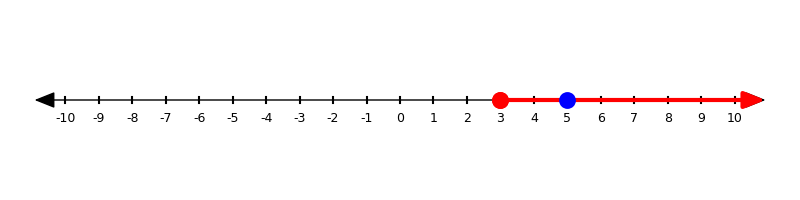
\includegraphics[width=1\linewidth,height=\textheight,keepaspectratio]{images/Glossary/greater_than_true.png}
but \(3 > 5\) is false
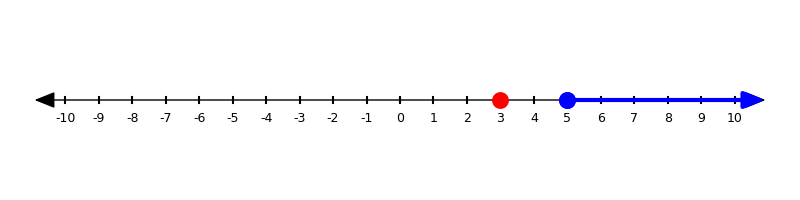
\includegraphics[width=1\linewidth,height=\textheight,keepaspectratio]{images/Glossary/greater_than_false.png}
\end{quote}

\begin{center}\rule{0.5\linewidth}{0.5pt}\end{center}

\subsection*{integer}\label{glossary-integer}
\addcontentsline{toc}{subsection}{integer}

In mathematics, an integer is a whole number (not a fraction or decimal)
that can be positive, negative, or zero. Examples include -3, 0, 5, and
100.

\begin{center}\rule{0.5\linewidth}{0.5pt}\end{center}

\subsection*{less than}\label{glossary-less-than}
\addcontentsline{toc}{subsection}{less than}

A number is less than (\textbf{\textless{}}) another number if it is
further to the left on the number line.

\begin{quote}
Example \(3 < 5\) is true
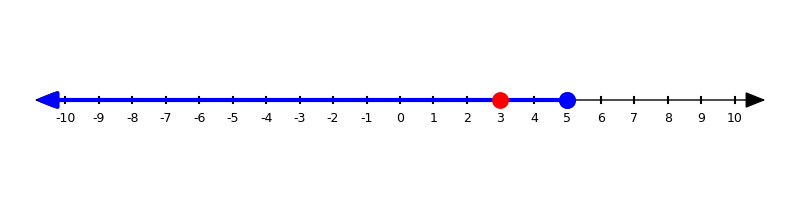
\includegraphics[width=1\linewidth,height=\textheight,keepaspectratio]{images/Glossary/less_than_true.png}
but \(5 < 3\) is false
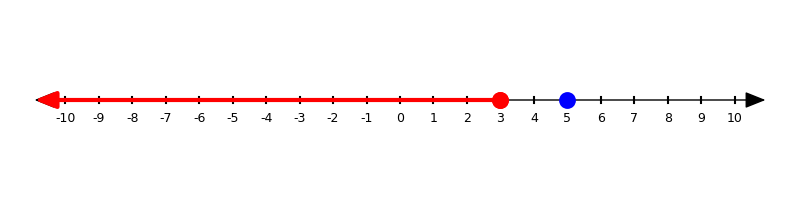
\includegraphics[width=1\linewidth,height=\textheight,keepaspectratio]{images/Glossary/less_than_false.png}
\end{quote}

\begin{center}\rule{0.5\linewidth}{0.5pt}\end{center}

\subsection*{number line}\label{glossary-number-line}
\addcontentsline{toc}{subsection}{number line}

A straight line used to represent numbers in order. It usually has zero
in the middle, with positive numbers to the right and negative numbers
to the left. Number lines help visualize operations and compare values.

\begin{quote}
Example: \(-2\), \(0\), and \(3\) are all on the number line.
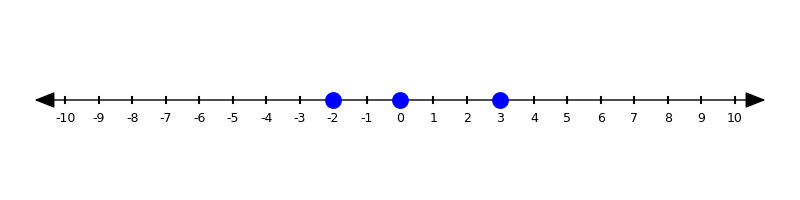
\includegraphics[width=1\linewidth,height=\textheight,keepaspectratio]{images/Glossary/number_line_example.png}
\end{quote}

\begin{center}\rule{0.5\linewidth}{0.5pt}\end{center}

\subsection*{negative number}\label{glossary-negative-number}
\addcontentsline{toc}{subsection}{negative number}

A number less than zero. On a number line, negative numbers are to the
left of zero.

\begin{quote}
Example: \texttt{-4} is a \textbf{negative number}.
\end{quote}

\begin{center}\rule{0.5\linewidth}{0.5pt}\end{center}

\subsection*{opposite}\label{glossary-opposite}
\addcontentsline{toc}{subsection}{opposite}

Two numbers that are the same distance from zero on a number line, but
on opposite sides. Their sum is always zero.

\begin{quote}
Example: \texttt{-3} and \texttt{3} are \textbf{opposite} numbers.
\end{quote}

\begin{center}\rule{0.5\linewidth}{0.5pt}\end{center}

\subsection*{positive number}\label{glossary-positive-number}
\addcontentsline{toc}{subsection}{positive number}

A number greater than zero. On a number line, positive numbers are to
the right of zero.

\begin{quote}
Example: \texttt{5} is a \textbf{positive number}.
\end{quote}

\begin{center}\rule{0.5\linewidth}{0.5pt}\end{center}




\end{document}
